\documentclass[11pt, aspectratio=169, xcolor={dvipsnames}]{beamer} %without handout s.t. one may use pause etc.; dauert aber etwas länger zum kompilieren...
\usepackage{tikz}
\usepackage{comment}
\usepackage{lmodern}
\usepackage{setspace}
\usepackage{hyperref}
\usepackage{array}
\usepackage[font=footnotesize]{subfig}
\usepackage[utf8]{inputenc}
\usetikzlibrary{arrows.meta,shapes,calc,shapes.geometric}
\usetikzlibrary{angles,quotes}
\usepackage{todonotes}
\usepackage[most]{tcolorbox}
\tcbuselibrary{theorems}
\usepackage{graphicx}
\usepackage{tabularx}

\tikzset{
	frage/.style = {rectangle, rounded corners, inner sep=10pt, fill=blue!8, draw=blue,  font=\fontsize{30}{25}\selectfont\sffamily, text centered},
	blitz/.style = {rectangle, rounded corners, fill=orange!20, draw=orange, font=\fontsize{30}{30}\selectfont\sffamily,  inner sep=10pt, text centered},
	blitzvortrag/.style={rectangle, rounded corners, fill=red!20, draw=red, font=\fontsize{30}{30}\selectfont\sffamily,  inner sep=10pt, text centered},
	gruppe/.style = {font=\fontsize{25}{25}\selectfont\sffamily, ellipse, fill=LimeGreen!30},
	titel/.style = {text centered, font=\fontsize{55}{55}\selectfont\sffamily},
	%every node/.style = {fill=white, font=\fontsize{25}{25}\selectfont\sffamily, align=center},
	dreieck/.pic = {
		\draw[scale=0.7, ForestGreen, thick, fill=LimeGreen!40] (0,0) -- (1.2, 0) --  (0, 2) -- cycle;
	},
	dreiecksp/.pic = {
		\draw[scale=0.7, ForestGreen, thick, fill=LimeGreen!40] (0,0) --  (-1.2,0) -- (0, 2) -- cycle;
	},
	dreieckmatt/.pic = {
		\draw[scale=0.7, ForestGreen, densely dotted, thick, fill=LimeGreen!20] (0,0) -- (1.2, 0) --  (0, 2) -- cycle;
	},
	dreieckspmatt/.pic = {
		\draw[scale=0.7, ForestGreen, densely dotted, thick, fill=LimeGreen!20] (0,0) --  (-1.2,0) -- (0, 2) -- cycle;
	},
	dreieckblau/.pic = {
		\draw[scale=0.7, Blue, thick, fill=ProcessBlue!40] (0,0) -- (1.2, 0) --  (0, 2) -- cycle;
	},
	dreiecklila/.pic = {
		\draw[scale=0.7, Violet, thick, fill=Thistle!40] (0,0) -- (-1.2, 0) --  (0, 2) -- cycle;
	},
	dreieckgruenblau/.pic = {
		\draw[scale=0.7, teal, thick, fill=Aquamarine!40] (0,0) -- (1.2, 0) --  (0, 2) -- cycle;
	},
	dreieckblausp/.pic = {
		\draw[scale=0.7, Orange, thick, fill=YellowOrange!40] (0,0) --  (-1.2,0) -- (0, 2) -- cycle;
	},
	spiegelpfeil/.pic = {
		\draw[thick, ->, fill=white]	(-1.5,0.40) to[out=305, in=165](0,0) arc(-95:275:.5) to [out=15, in=215](1.5,0.4);
	},
	spiegelpfeilrot/.pic = {
		\draw[thick, ->, red, fill=white]	(-1.5,0.40) to[out=305, in=165](0,0) arc(-95:275:.5) to [out=15, in=215](1.5,0.4);
	},
	fahne/.pic = {
		\draw[thick]	(0,0) -- (1.4, 0) -- (1.2, 0.2) -- (1,0);
	},
	fahneunten/.pic = {
		\draw[thick]	(0,0) -- (1.4, 0) -- (1.2, -0.2) -- (1,0);
	},
	fahnelinks/.pic = {
		\draw[thick]	(0,0) -- (-1.4, 0) -- (-1.2, 0.2) -- (-1,0);
	},
	fahnerotiert/.pic = {
		\draw[thick]	(0,0) -- (-1.4, 0) -- (-1.2, -0.2) -- (-1,0);
	},
	dreh2pink/.pic = {
		\draw[thick, fill=magenta, scale=0.2] (-0.5,0) -- (0,1) -- (0.5,0) -- (0,-1) -- cycle;
	},
	dreh2blue/.pic = {
		\draw[thick, fill=blue, scale=0.2] (-0.5,0) -- (0,1) -- (0.5,0) -- (0,-1) -- cycle;
	},
	dreh2LimeGreen/.pic = {
		\draw[thick, fill=LimeGreen, scale=0.2] (-0.5,0) -- (0,1) -- (0.5,0) -- (0,-1) -- cycle;
	},
	dreh2orange/.pic = {
		\draw[thick, fill=orange, scale=0.2] (-0.5,0) -- (0,1) -- (0.5,0) -- (0,-1) -- cycle;
	},
	dreh3/.pic = {
		\draw (0,0) node[regular polygon, regular polygon sides=3, inner sep=0.06cm, thick, fill=red, draw=black] {};
	},
	dreh4/.pic = {
		\draw (0,0) node[regular polygon, regular polygon sides=4, inner sep=0.07cm, thick, fill=LimeGreen, draw=black] {};
	},
	dreh6/.pic = {
		\draw (0,0) node[regular polygon, regular polygon sides=6, inner sep=0.08cm, thick, fill=blue, draw=black] {};
	},
}


\newcommand{\NN}{\mathbb{N}}
\newcommand{\ZZ}{\mathbb{Z}}
\newcommand{\red}{\textcolor{red}}
\newcommand{\blue}{\textcolor{blue}}
\newcommand{\green}{\textcolor{ForestGreen!80!black}}
\newcommand{\white}{\textcolor{white}}
\definecolor{beamerblue}{RGB}{9, 67, 124}
\newcommand{\beamerblue}{\textcolor{beamerblue}}
\definecolor{beamergreen}{RGB}{0, 150, 20}
\newcommand{\beamergreen}{\textcolor{beamergreen}}

\def\me{\mathcal{E}}
\def\mk{\mathcal{K}}

\DeclareMathOperator{\sgn}{sgn}
\DeclareMathOperator{\id}{id}

\theoremstyle{plain}
\newtheorem{satz}{Satz}
\newtheorem{kor}[satz]{Folgerung}

\theoremstyle{definition} 
\newtheorem{Def}[satz]{Definition}

%\tcolorboxenvironment{satz}{
	%	colback=Cyan!15,  %Green!15,
	%	colframe=beamerblue,  %Green!80!Blue,
	%	%blanker, 
	%	breakable,left=5mm,
	%	before skip=10pt,after skip=10pt,
	%	%borderline west={1mm}{0pt}{orange}
	%}

\mode<presentation>{
	%	\useinnertheme{circles}
	\usetheme{Boadilla}
	\usecolortheme[RGB={9,67,124}]{structure}
	%	\usecolortheme{whale}
	%	\usecolortheme{orchid}
	\beamertemplatenavigationsymbolsempty
	%	\setbeamercolor{alerted text}{fg=blue}
	%	\renewcommand{\thefootnote}{\fnsymbol{footnote}}
	\setbeamertemplate{frametitle}[default][center] %zentrierte Titel
	\setbeamercovered{invisible} %covered space is invisible and not only shaded
}

%\newtcolorbox{aufgabenbox}
%{
%	colback  = BurntOrange!20, 
%	colframe = BurntOrange!20, 
%	left=1pt
%}
%
%\newtcolorbox{satzbox}
%{
%	colback=Cyan!15,  %Green!15,
%	colframe=beamerblue,  %Green!80!Blue,
%	%blanker, 
%	breakable,left=2mm,
%	before skip=10pt,after skip=10pt,
%	%borderline west={1mm}{0pt}{orange}
%}
%\newtcolorbox{defbox}
%{
%	colback  = green!15, 
%	colframe = green!15, 
%	left=1pt
%}

\newtcbtheorem{defbox}{Definition} 
{ enhanced jigsaw,colframe=ForestGreen!80,%interior hidden, %vorher war Blue!60
	breakable,before skip=10pt,after skip=10pt
}{} %options

\newtcbtheorem{satzbox}{Satz} 
{ enhanced jigsaw,colframe=Plum!80,%interior hidden, %vorher war Blue!60
	breakable,before skip=10pt,after skip=10pt
}{} %options

\newtcbtheorem{lemmabox}{Lemma (Hilfssatz)} 
{ enhanced jigsaw,colframe=Plum!80,%interior hidden, %vorher war Blue!60
	breakable,before skip=10pt,after skip=10pt
}{}

\newtcbtheorem{folgbox}{Folgerung} 
{ enhanced jigsaw,colframe=Plum!80,%interior hidden, %vorher war Blue!60
	breakable,before skip=10pt,after skip=10pt
}{} %options

\newtcolorbox{aufgabenbox}
{
	colback  = Orange!20, 
	colframe = Orange!20, 
	left=1pt
}

\newtcolorbox{rememberbox}
{
	colback  = Yellow!20, 
	colframe = Yellow!20, 
	left=1pt
}


\newtcolorbox{greenbox}
{
	%colback  = ForestGreen!80, 
	colframe = ForestGreen!80, 
	left=1pt
}


\title{Workshops für Schülerinnen und Schüler}
\author{Dr. Anna Schilling}

%\institute{Forschungsstelle Geometrie + Dynamik}

\subtitle{}
\date{17.3.2026}

%
\includegraphics{Bilder/GEODYN-Logo_RGB.png}}

\begin{document}


\begin{frame}
	\titlepage
\end{frame}

\begin{frame}
	\begin{center}
		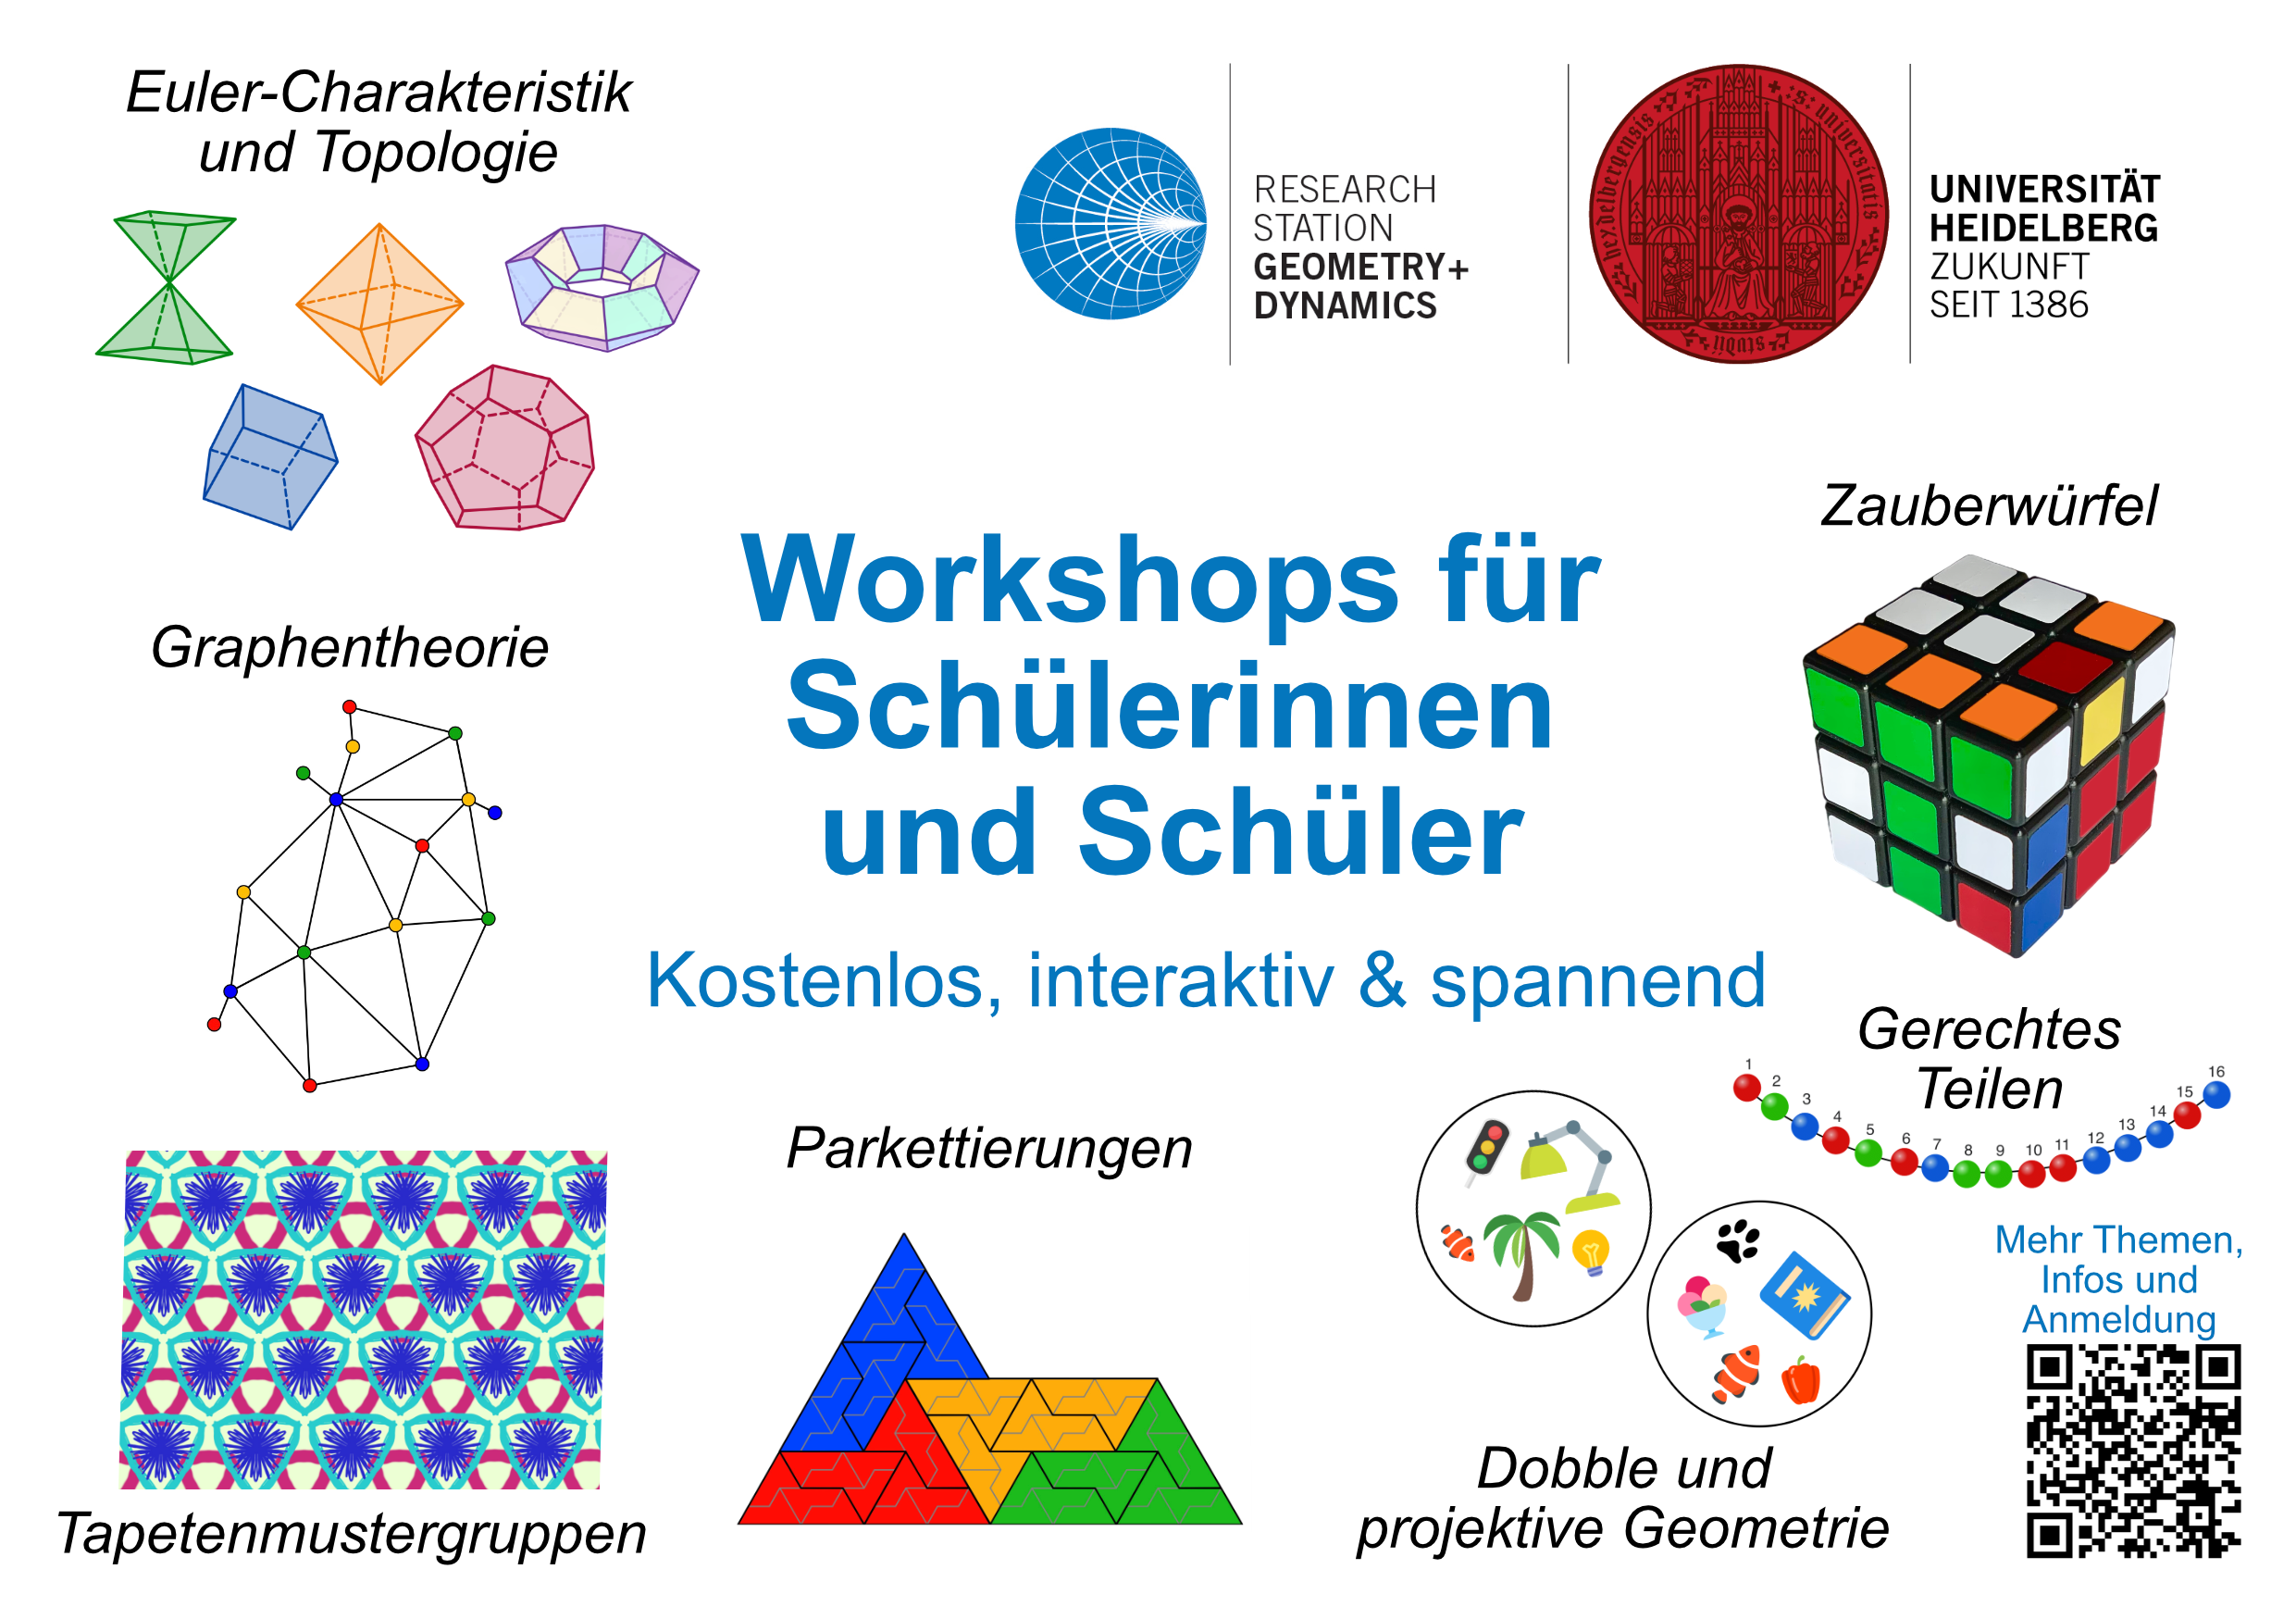
\includegraphics[height=\textheight]{Bilder/Flyer.png}
	\end{center}
\end{frame}

\begin{frame}
	\centering
	%\Large{\beamerblue{Teil 1:}}
	\Large{\beamerblue{Unsere Workshops}}
\end{frame}

\begin{frame}{Euler-Charakteristik und Topologie \\ \small{Unterstufe - Mittelstufe}}
	\begin{minipage}{0.6\textwidth}
		Inhalt:
		\begin{itemize}
			\item Eulersche Polyederformel 
			\item Euler-Charakteristik von planaren Graphen
			\item Der Eulersche Polyedersatz für konvexe Polyeder
			\item Topologie und Invarianten
		\end{itemize}
		
		\hfill
		
		Mathematik:
		\begin{itemize}
			\item Planare Graphen 
			\item Konvexe Polyeder
			\item Stereographische Projektion 
			\item Beweis der Polyederformel
			\item Ideen der Topologie und Invarianten
		\end{itemize}
	\end{minipage}
	\begin{minipage}{0.38\textwidth}
		\centering
		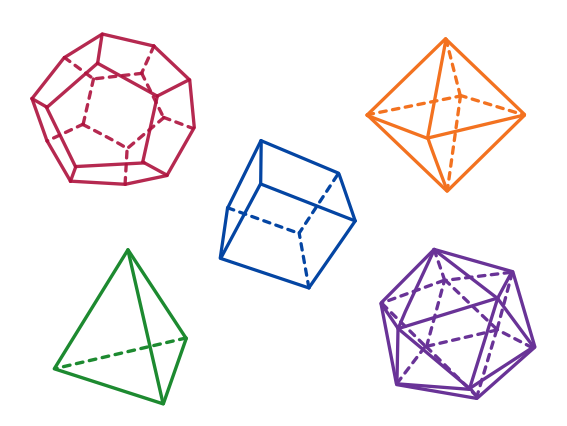
\includegraphics[width=0.9\textwidth]{Bilder/Platonische-Koerper.png} \\[4pt]
		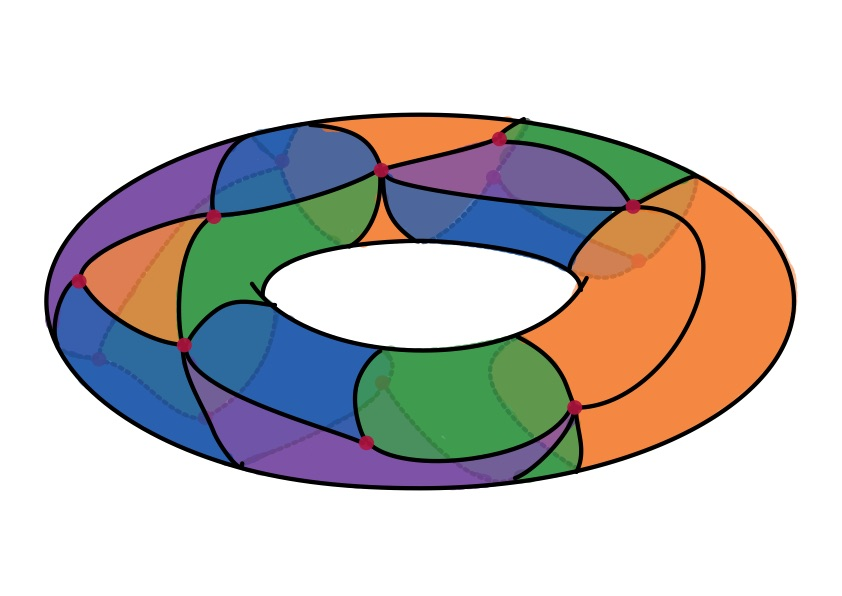
\includegraphics[width=0.7\textwidth]{Bilder/Torus.jpg}
	\end{minipage}
\end{frame}

\begin{frame}{Parkettierungen\\ \small{Unterstufe - Mittelstufe - Oberstufe}}
	\begin{minipage}{0.6\textwidth}
		Inhalt: 
		\begin{itemize}
			\item Regelmäßige Parkettierungen
			\item Parkettierungen mit allgemeinen 3- und 4-Ecken
			\item Parkettierungen mit 5-Ecken
			\item Aperiodische Parkettierungen (Penrose, Einstein)
			\item Sphärische und hyperbolische Parkettierungen
		\end{itemize}
		
		\hfill
		
		Mathematik:
		\begin{itemize}
			\item Innenwinkelsumme im \(n-\)Ecke
			\item Beweisidee Aperiodizität
			\item Nicht-Euklidische Geometrien
		\end{itemize}
	\end{minipage}
	\begin{minipage}{0.38\textwidth}
		\centering
		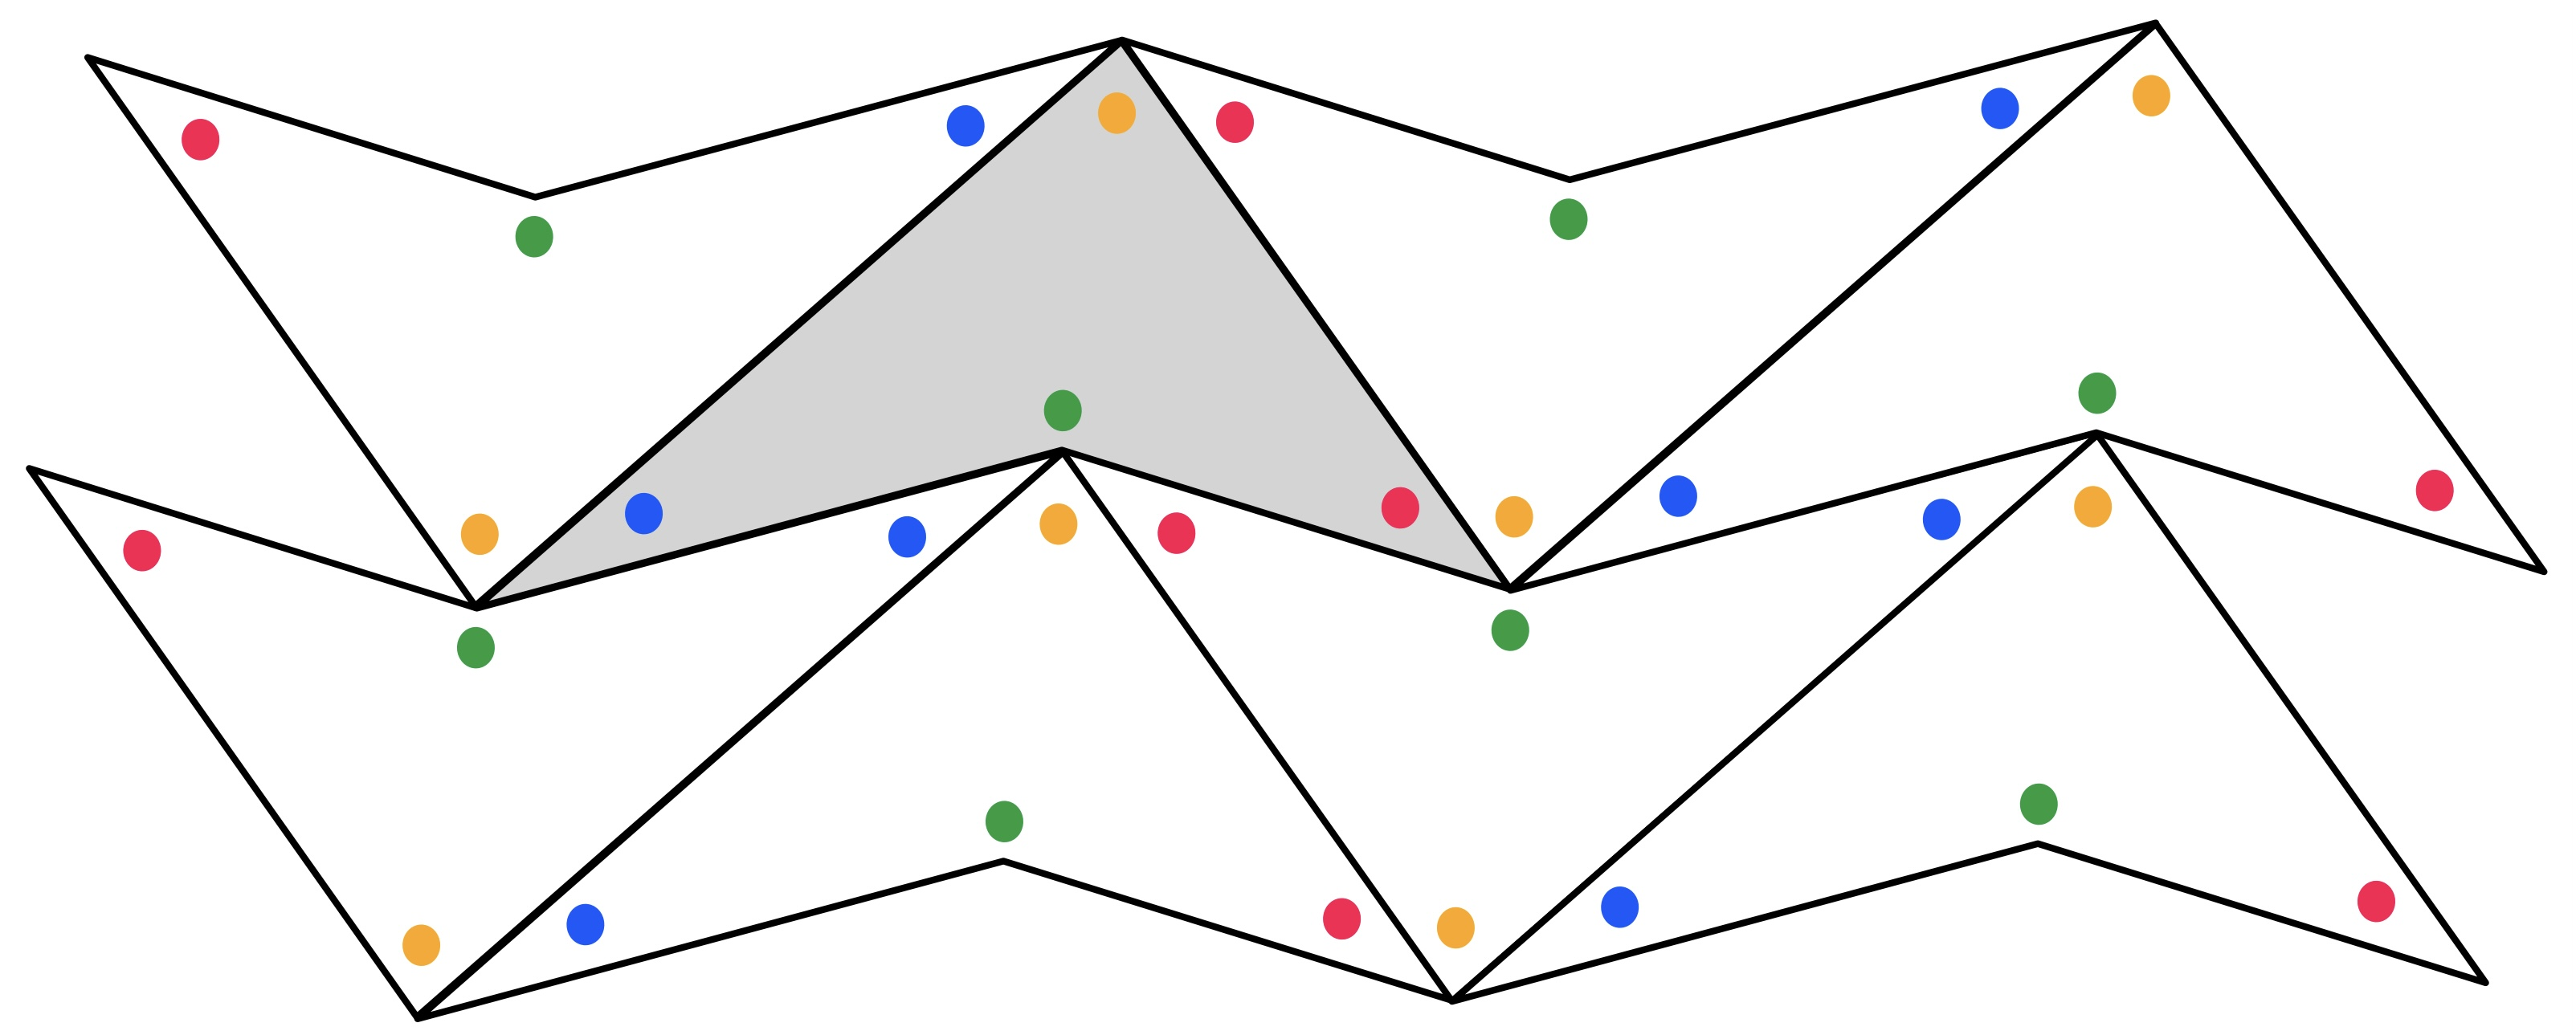
\includegraphics[width=0.9\textwidth]{Bilder/Resultat_Viereck_konkav_Abschlussfolie.jpeg}\\[13pt]
		
		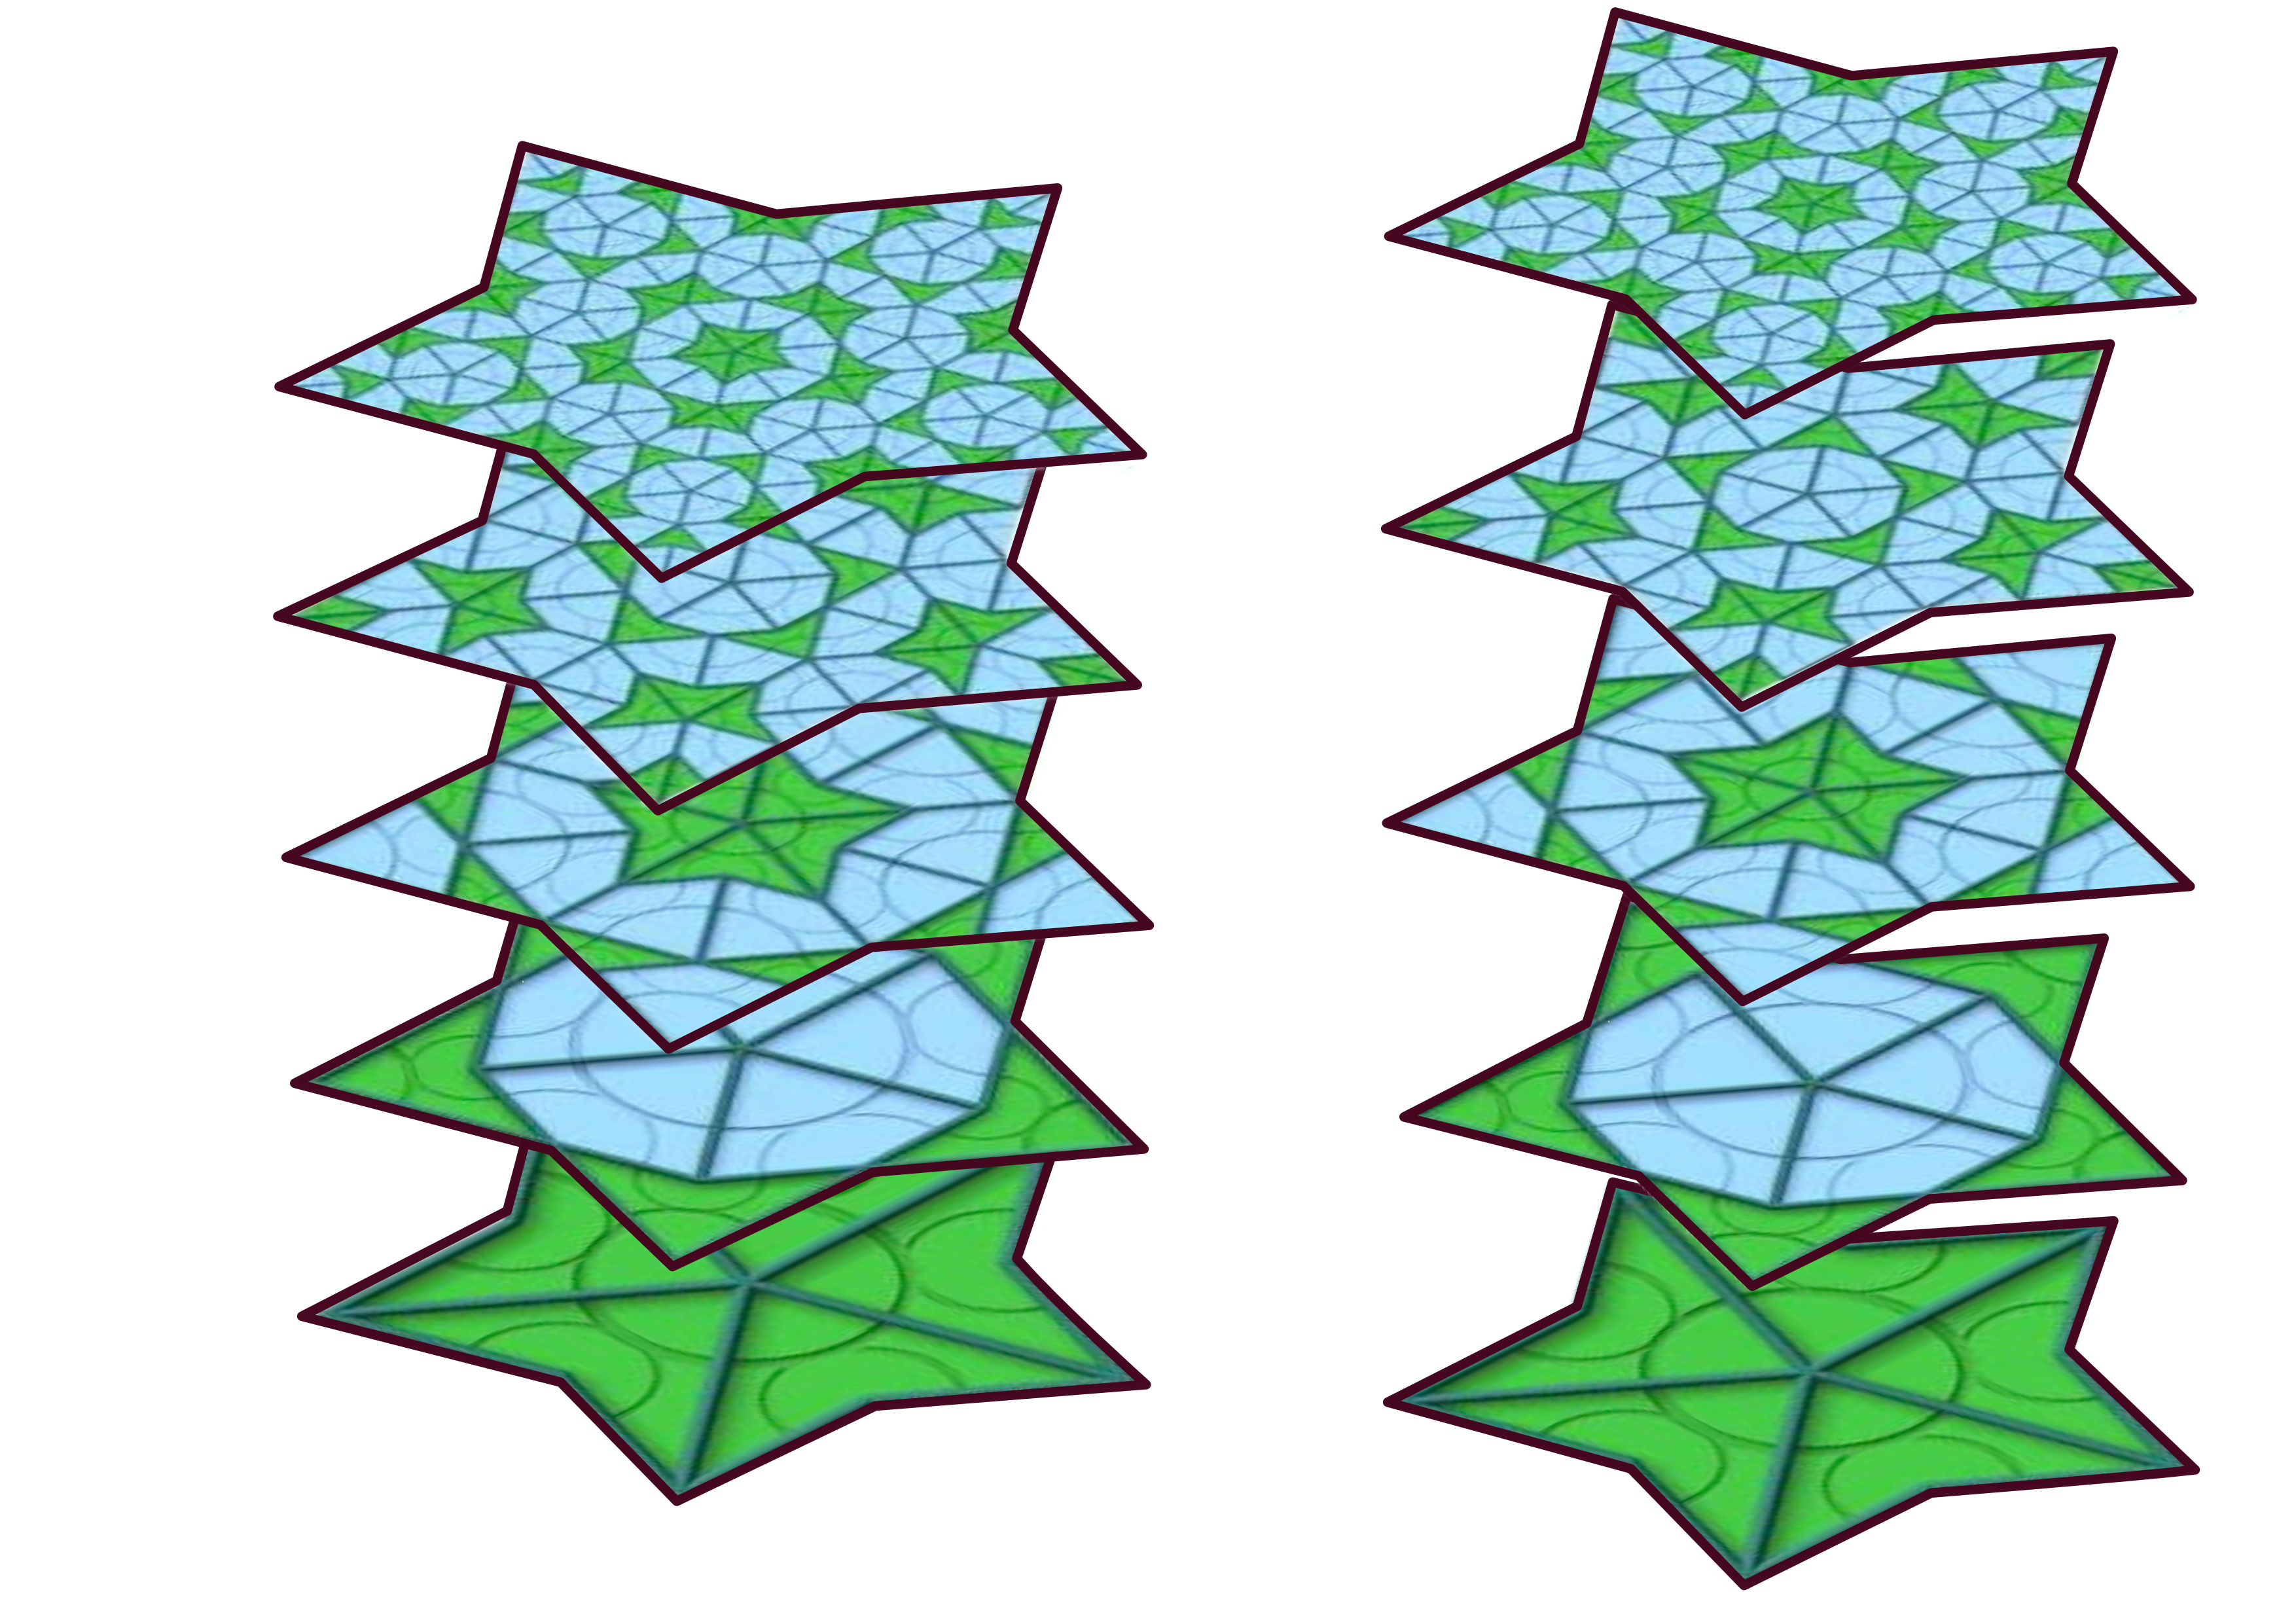
\includegraphics[height=0.4\textheight]{Bilder/Penrose_Stapel_umrandet_hoch.png}
	\end{minipage}
\end{frame}

\begin{frame}{Tapetenmustergruppen\\ \small{Unterstufe - Mittelstufe - Oberstufe}}
	\begin{minipage}{0.6\textwidth}
		Inhalt: 
		\begin{itemize}
			\item Kongruenzabbildungen und Symmetrien
			\item Verknüpfung von Kongruenzabbildungen
			\item Tapetenmustergruppe
			\item Warum es nur 17 Tapetenmustergruppen gibt
		\end{itemize}
		
		\hfill
		
		Mathematik:
		\begin{itemize}
			\item Kongruenzabbildungen und Symmetrien
			\item Verknüpfung von Kongruenzabbildungen
			\item Gruppen
			\item Beweis über Ausschlussprinzip (Flowchart)
		\end{itemize}
	\end{minipage}
	\begin{minipage}{0.38\textwidth}
		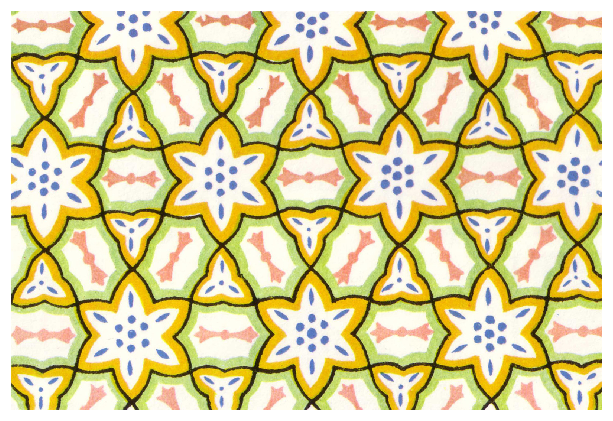
\includegraphics[height=0.55\textheight, angle=90]{Bilder/Blumenbeispiel_Standalone_leer.pdf}
	\end{minipage}
\end{frame} 

\begin{frame}{Graphentheorie\\ \small{Unterstufe - Mittelstufe - (Oberstufe})}
	\begin{minipage}{0.3\textwidth}
		Inhalt: 
		\begin{itemize}
			\item Graphen
			\item Planare Graphen
			\item Färbung von Graphen
			\item Euler-Kreise
		\end{itemize}
		
		\hfill
		
		Mathematik:
		\begin{itemize}
			\item Triangulierungen
			\item Beweistechniken
		\end{itemize}
	\end{minipage}
	\begin{minipage}{0.68\textwidth}
		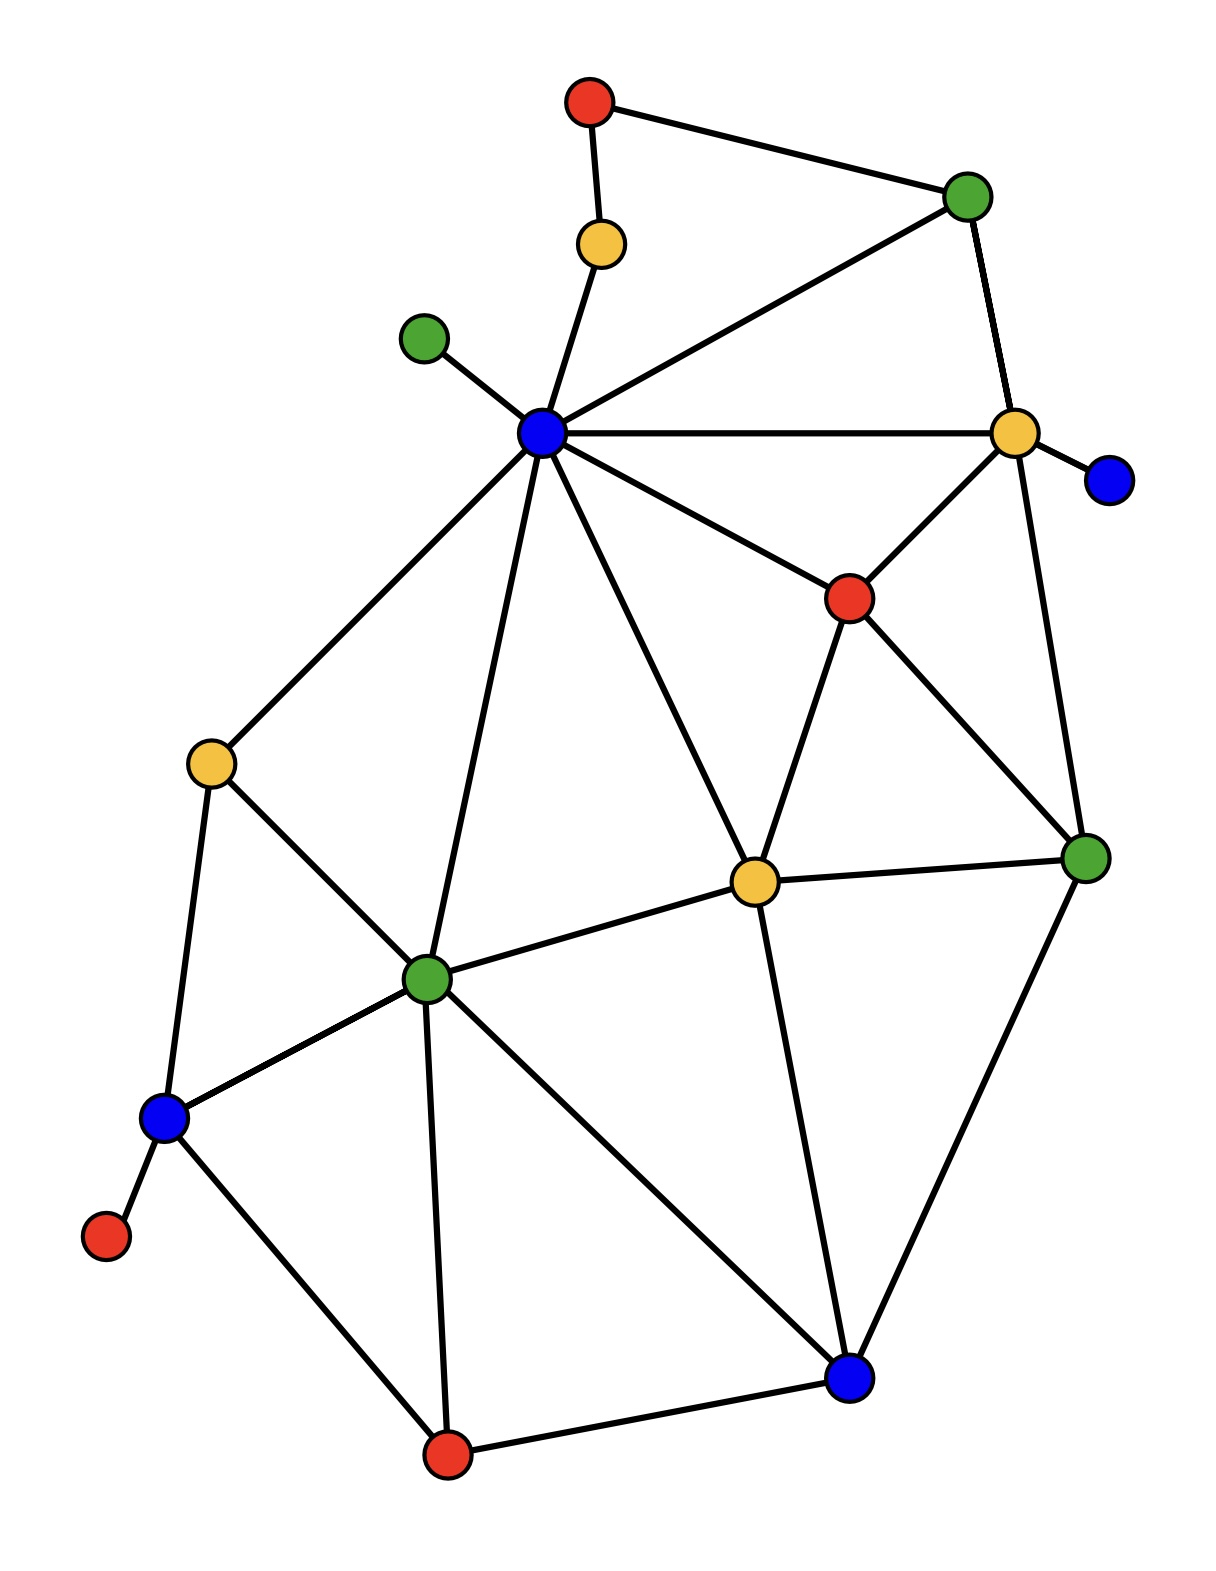
\includegraphics[width=0.4\textwidth]{Bilder/Graph.jpg} \quad
		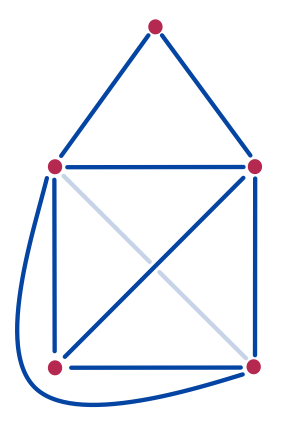
\includegraphics[width=0.4\textwidth]{Bilder/Haus-Nikolaus.png}
	\end{minipage}
\end{frame}


\begin{frame}{Gerechtes Teilen\\ \small{Unterstufe - Mittelstufe - Oberstufe}}
	\begin{minipage}{0.6\textwidth}
		Inhalt: 
		\begin{itemize}
			\item Was heißt "gerecht"?
			\item Gerechtes Teilen einer Perlenkette
			\item Protokolle für gerechte Kuchenteilung
			\item Das Sperner-Lemma
		\end{itemize}
		
		
		
		\phantom{A}
		
		
		Mathematik:
		\begin{itemize}
			\item Funktionen
			\item Protokoll (Fallunterscheidungen + Abstraktion)
			\item Beweisstrukturen
		\end{itemize}
	\end{minipage}
	\begin{minipage}{0.38\textwidth}
		\centering
		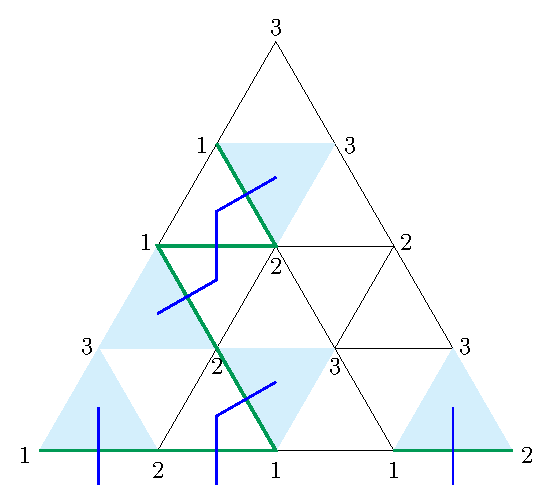
\includegraphics[height=0.5\textheight]{Bilder/Dreieck_Beschriftung_Beispiel_Raeume.pdf}\\[3pt]
		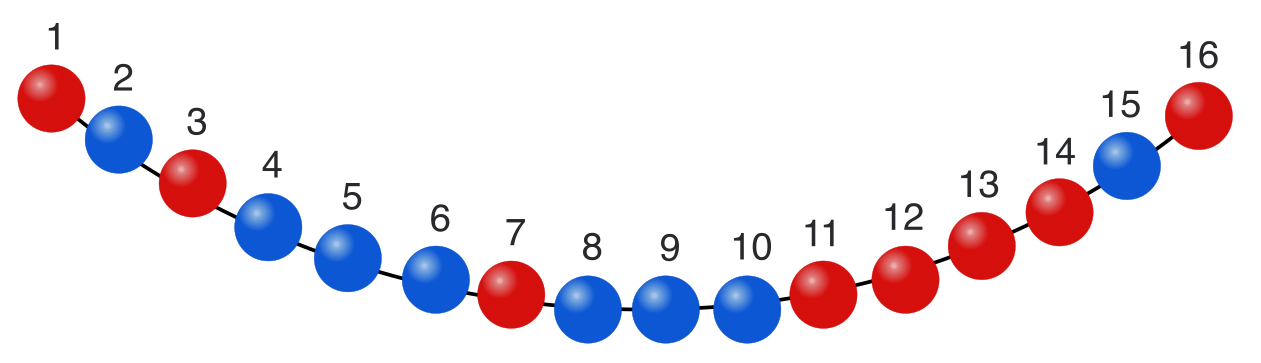
\includegraphics[width=0.9\textwidth]{Bilder/Perlenkette_gebogen.png}
	\end{minipage}
\end{frame}



\begin{frame}{Dobble und Projektive Geometrie\\ \small{(Unterstufe) - Mittelstufe - Oberstufe}}
	\begin{minipage}{0.65\textwidth}
		Inhalt: 
		\begin{itemize}
			\item Das Spiel Dobble 
			\item Ideale Dobble-Spiele
			\item (Ebene) projektive Geometrie
			\item Existenz von Dobble-Spielen
		\end{itemize}
		
		\hfill
		
		Mathematik:
		\begin{itemize}
			\item Eigenschaften idealer Dobble-Spiele
			\begin{itemize}
				\item Symbole pro Karte = Häufigkeit der Symbole
				\item Anzahl aller Karten = Anzahl aller Symbole
			\end{itemize}
			\item Idee projektive Geometrie
			\item Eigenschaften endlicher projektiver Ebenen
			\item Struktur mathematischer Aussagen
		\end{itemize}
	\end{minipage}
	\begin{minipage}{0.33\textwidth}
		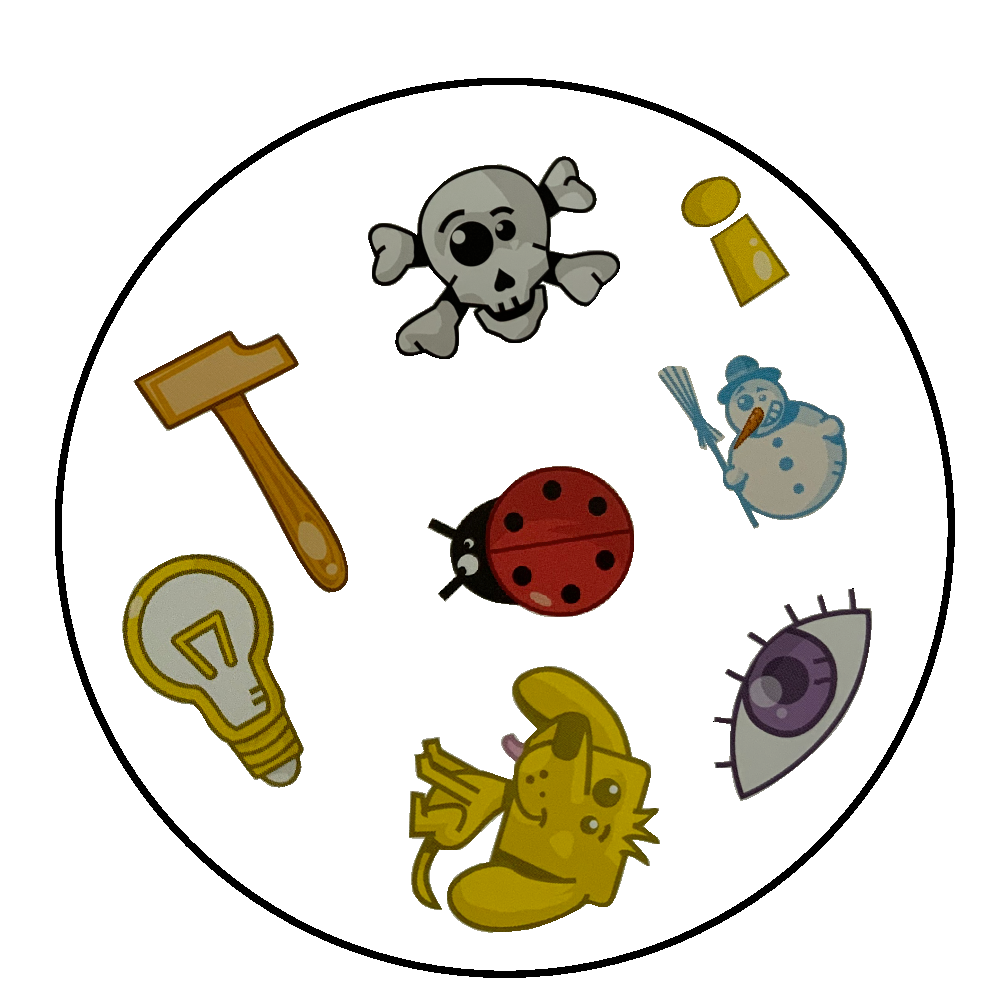
\includegraphics[height=0.4\textheight]{Bilder/Karte1.pdf}\\ 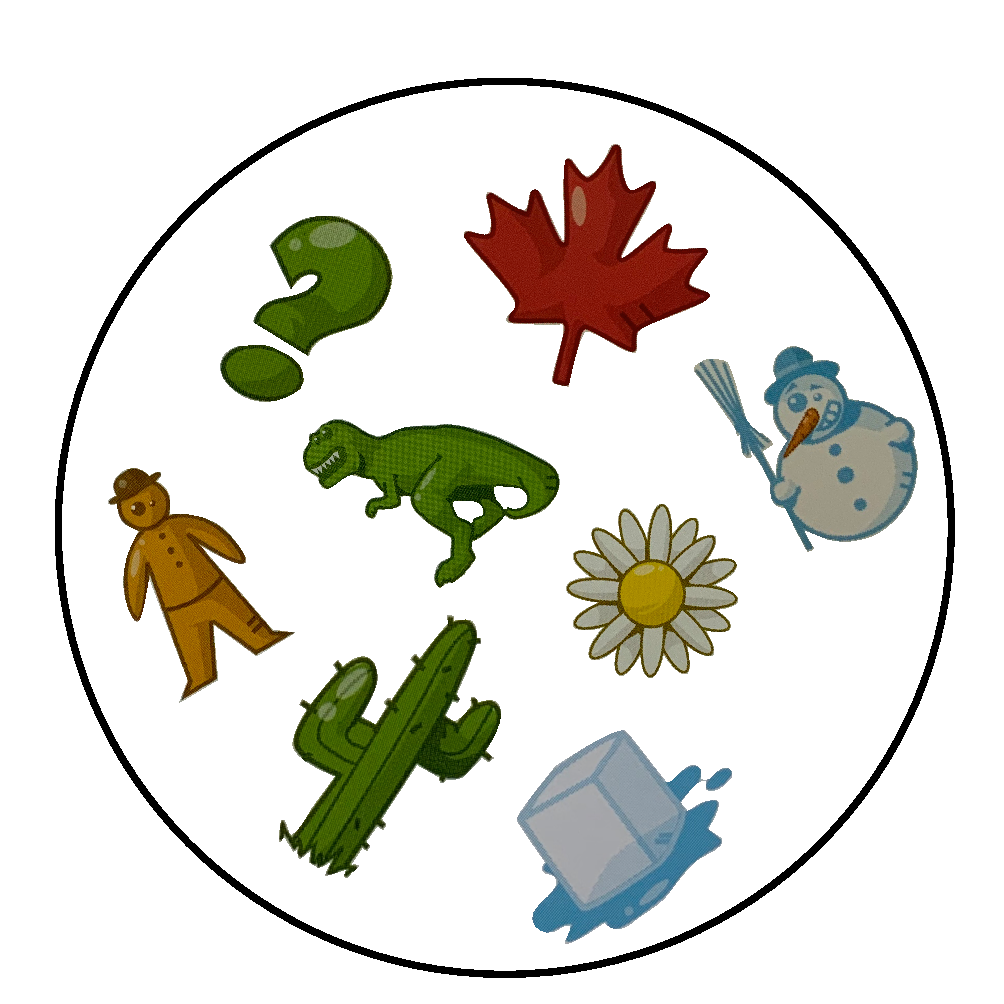
\includegraphics[height=0.4\textheight]{Bilder/Karte2.pdf}
	\end{minipage}
\end{frame}

\begin{frame}{Zauberwürfel und Gruppentheorie\\ \small{Oberstufe}}
	\begin{minipage}{0.6\textwidth}
		Inhalt: 
		\begin{itemize}
			\item Der Zauberwürfel und Drehungen 
			\item Gruppe der Vertauschungen
			\item Mathematische Beschreibung des Zauberwürfels
			\item Lösbarkeitssatz
		\end{itemize}
		
		\hfill
		
		Mathematik:
		\begin{itemize}
			\item Gruppen allgemein
			\item Symmetrische Gruppe und Zykel
			\item Abstrakte Würfelbeschreibung
			\item Beweis des Lösbarkeitssatzes
		\end{itemize}
	\end{minipage}
	\begin{minipage}{0.38\textwidth}
		\centering
		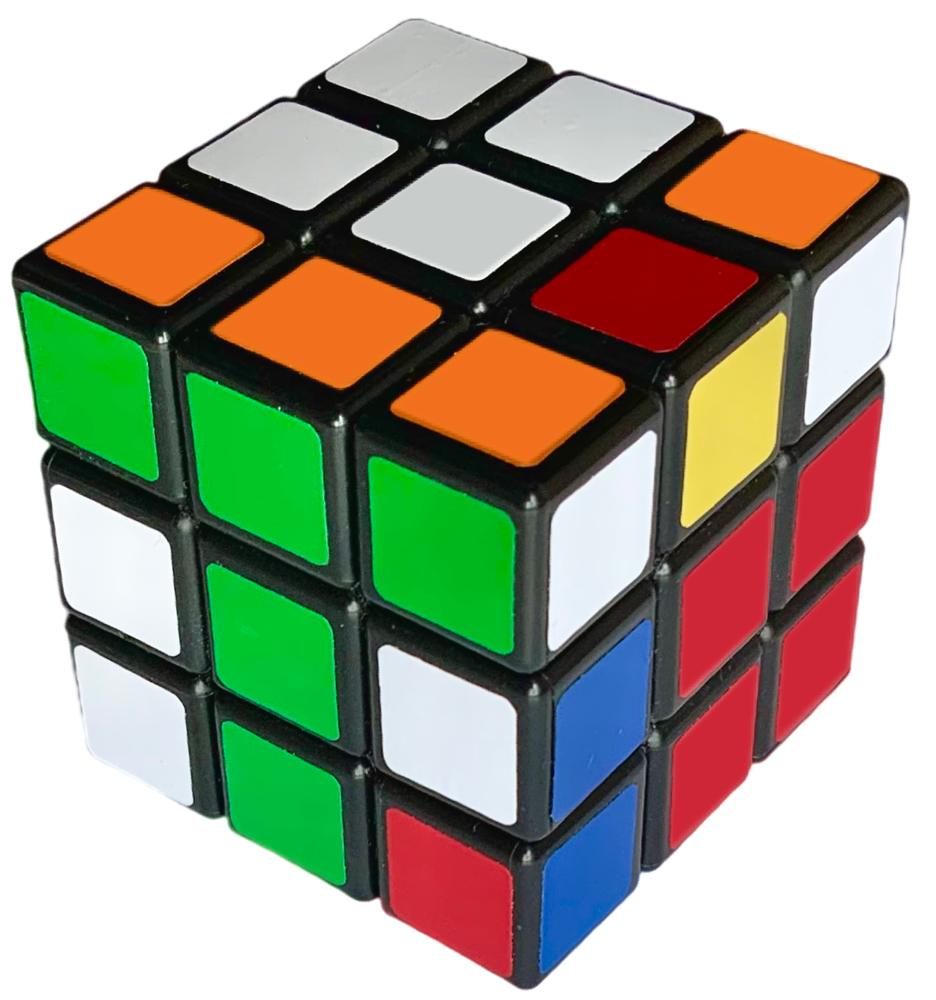
\includegraphics[height=0.35\textheight]{Bilder/Wuerfel_gerade_ausgeschnitten.png}\\[3pt]
		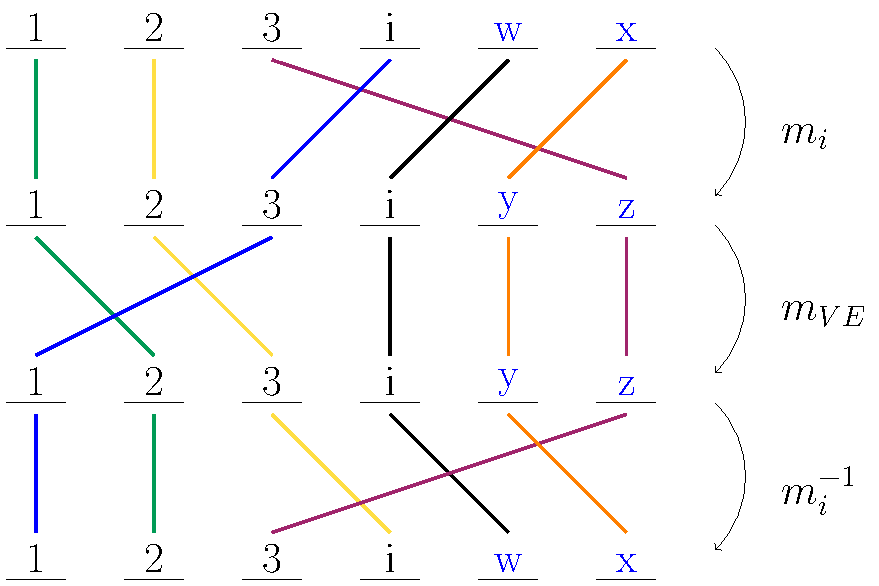
\includegraphics[height=0.4\textheight]{Bilder/Zykel.pdf}
	\end{minipage}
\end{frame}



\begin{frame}
	\centering
	\Large{Teil 2:}\\[20pt]
	\Large{Konkrete Beispiele}
\end{frame}

\begin{frame}{Dobble und projektive Geometrie}
	\begin{figure}[h!]
		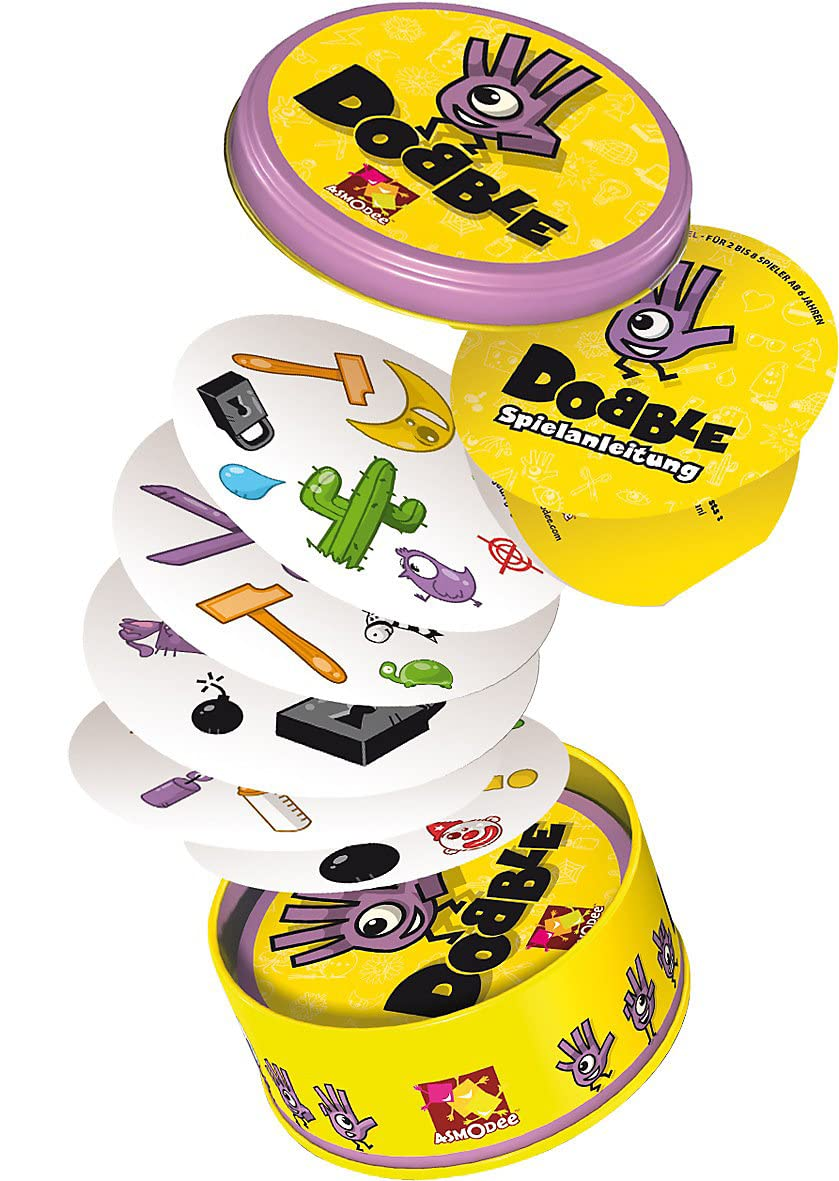
\includegraphics[height=0.75\textheight]{Bilder/Dobble-Spiel-original.jpg} 
		\quad \quad
		\begin{tikzpicture}
			\draw[ultra thick, <->] (-1, 3) -- (2,3);
			\coordinate[label=above: {\huge{?}}] (f) at (0.5, 3.2);
			\coordinate[label=above: {\textcolor{white}{.}}] (g) at (0,0);
		\end{tikzpicture}
		\quad \quad
		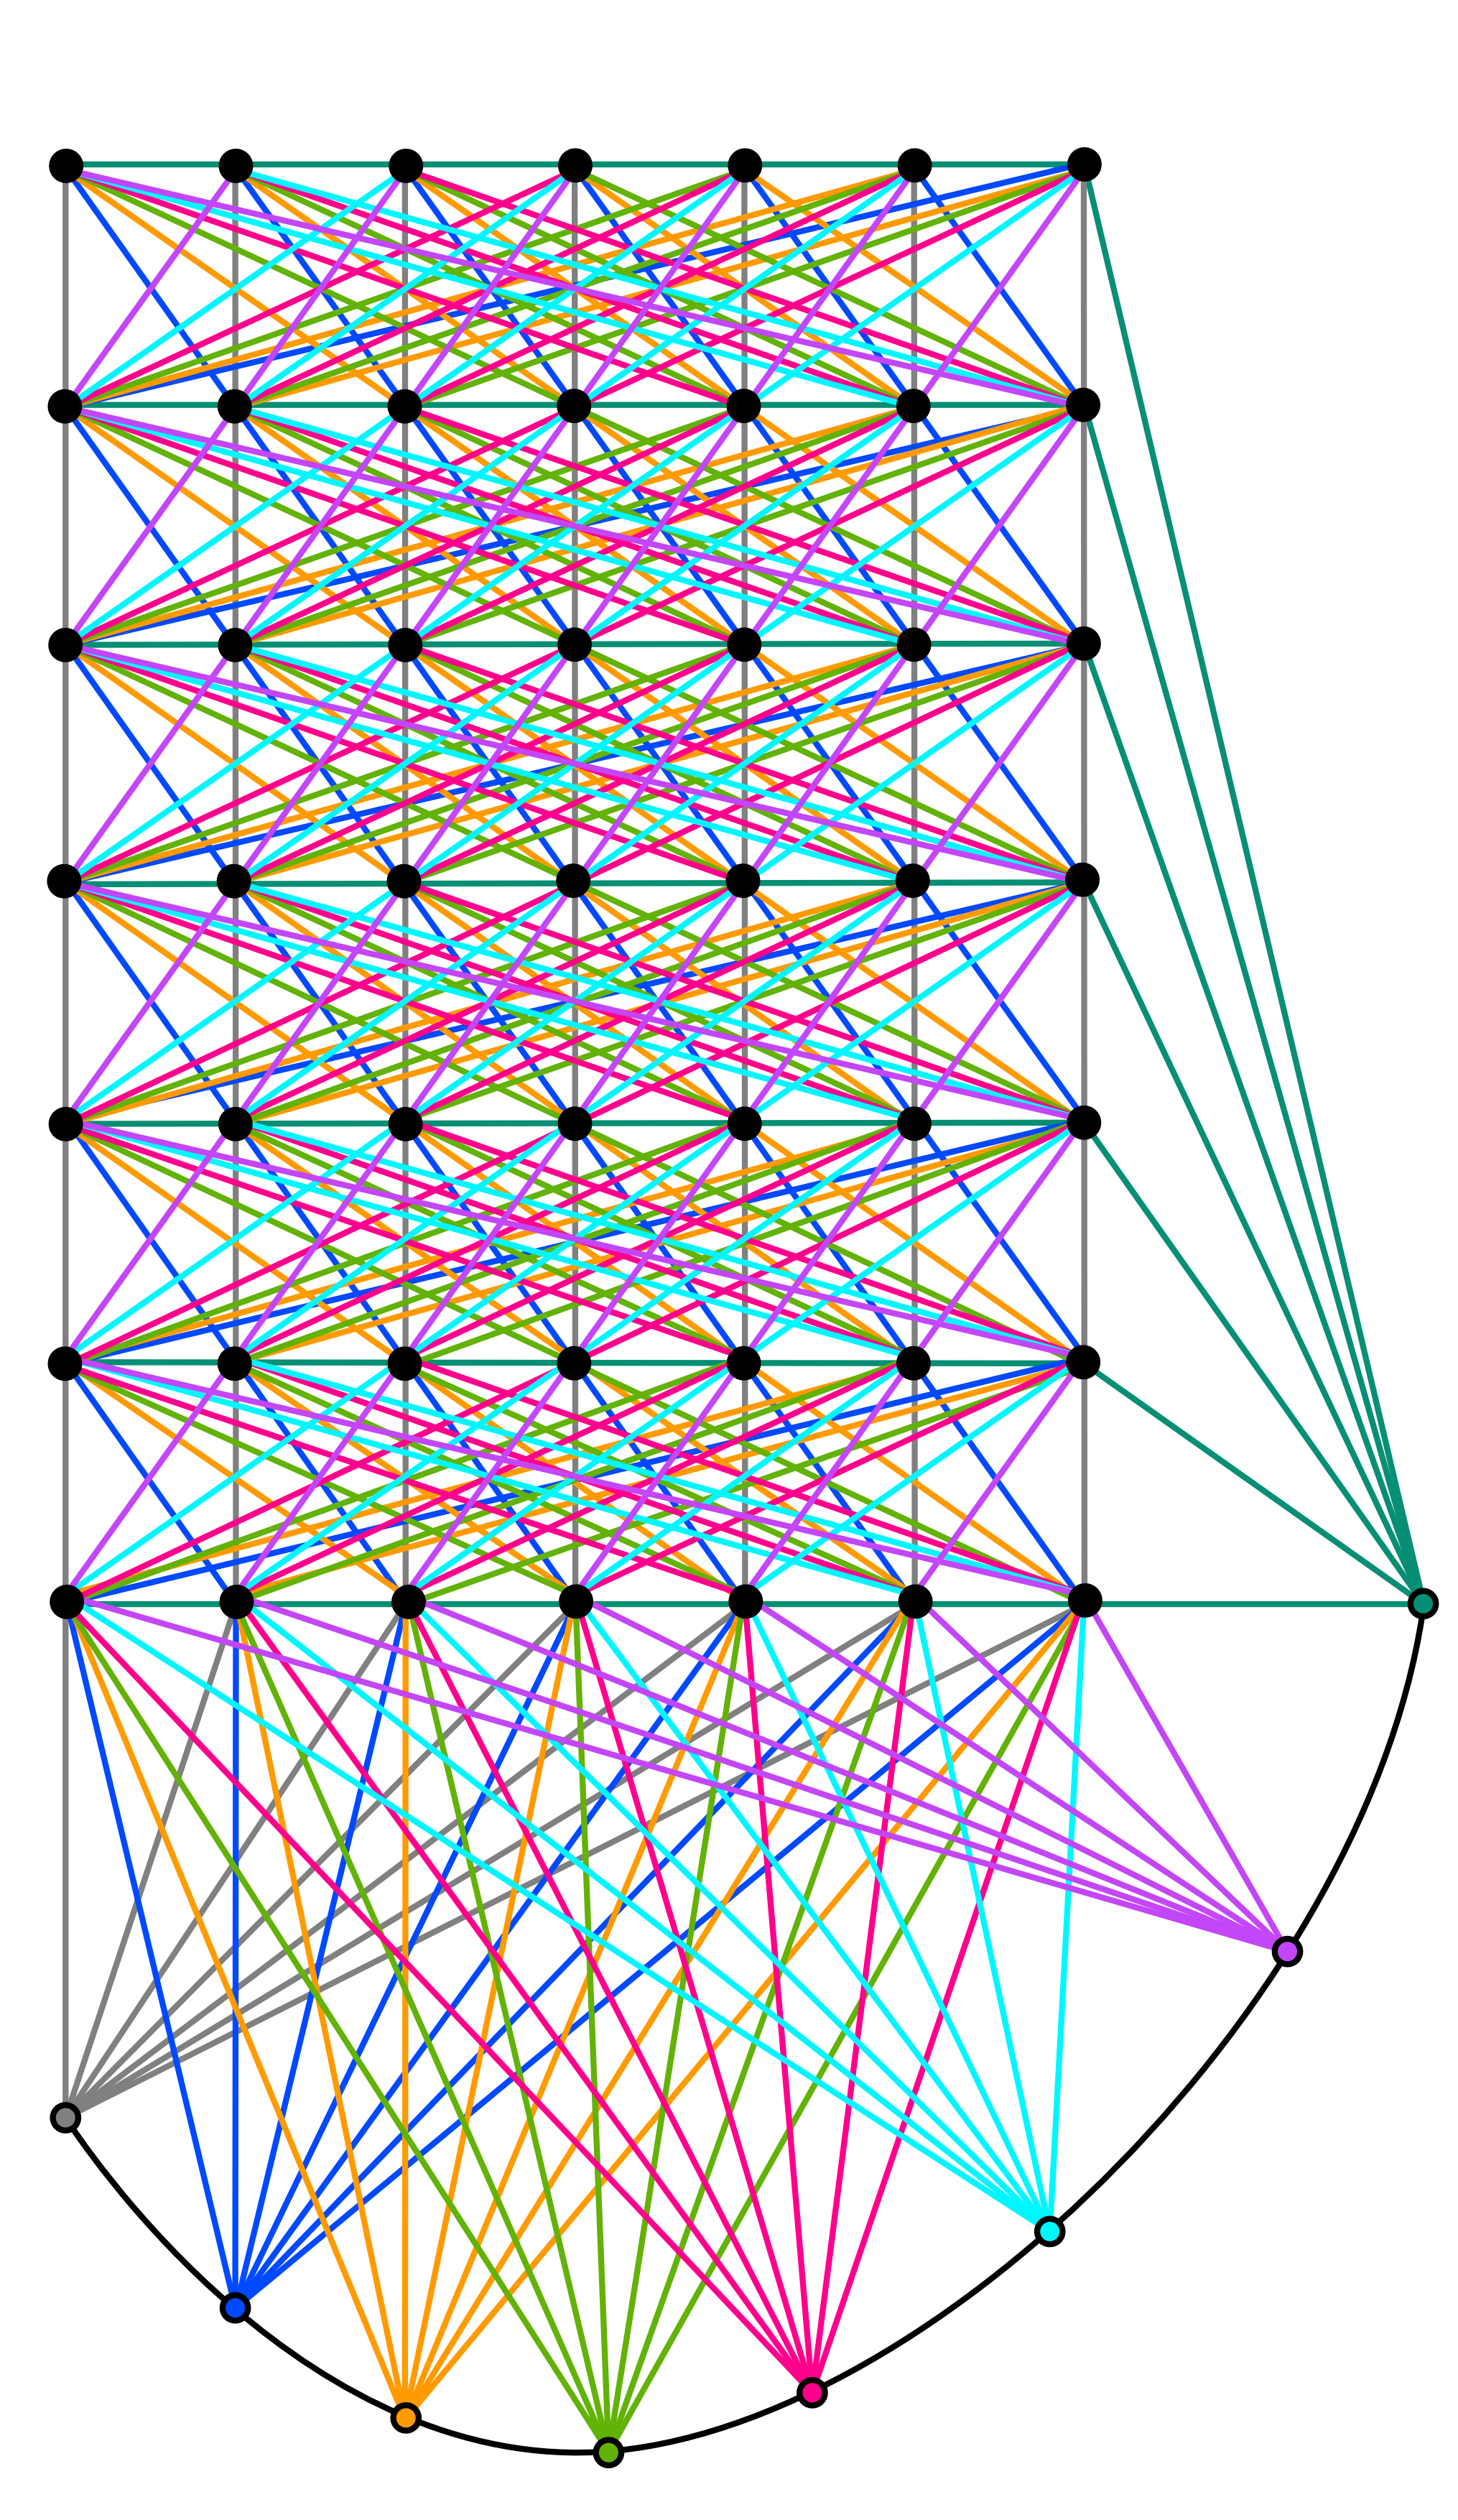
\includegraphics[height=0.75\textheight]{Bilder/Dobble-Ordnung-7-vollstaendig.png}
	\end{figure}
\end{frame}


\begin{frame}{Dobble}
	\begin{defbox*}{}{}
		Ein ideales Dobble-Spiel ist eine Ansammlung von Karten mit Symbolen darauf, sodass Folgendes gilt:
		\setbeamercolor{item projected}{bg=beamerblue,fg=white} %für Farbe, vorher Blue!60
		\setbeamertemplate{enumerate items}[circle]
		\begin{enumerate}%[label=\large\protect\textcircled{\small\arabic*}]
			\item Die Anzahl der Symbole pro Karte ist immer gleich.
			\item Jedes Symbol kommt gleich häufig vor.
			\item Je zwei Karten haben immer genau ein Symbol gemeinsam.
			\item Je zwei Symbole definieren immer genau eine Karte.
		\end{enumerate}
	\end{defbox*}
\end{frame}


\begin{frame}{Ein ganz einfaches Dobble-Spiel}
	\begin{center}
		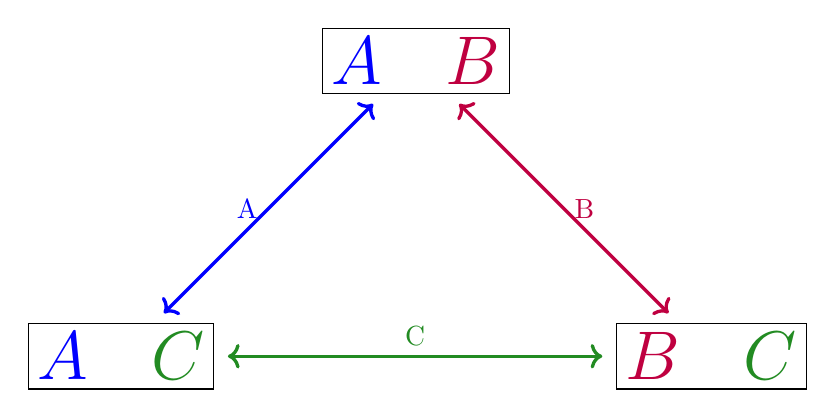
\begin{tikzpicture}[scale=2.5]
			\node at (0,1.5) [rectangle,draw] (k1) {\Huge{$\textcolor{blue}{A} \quad \textcolor{purple}{B}$}};
			\node at (-1.5, 0) [rectangle, draw] (k2) {\Huge{\(\textcolor{blue}{A} \quad \textcolor{ForestGreen}{C}\)}};
			\node at (1.5, 0) [rectangle, draw] (k3) {\Huge{\(\textcolor{purple}{B} \quad \textcolor{ForestGreen}{C}\)}};
			\draw[very thick, <->, shorten <=5pt, shorten >=5pt, blue] (k1) -- node[left, pos=0.5] {A} (k2);
			\draw[very thick, <->, shorten <=5pt, shorten >=5pt, purple] (k1) -- node[right, pos=0.5] {B} (k3);
			\draw[very thick, <->, shorten <=5pt, shorten >=5pt, ForestGreen] (k2) -- node[above, pos=0.5] {C} (k3);
		\end{tikzpicture}
	\end{center}
\end{frame}

\begin{frame}{Aufgabe}
	\begin{center}	
		Entwerft in der Gruppe ein Dobble-Spiel mit 3 Symbolen pro Karte. \\[10pt]
		Überlegt euch zuerst, wie viele Karten ihr braucht. 
	\end{center}
	
	
	\vfill
	
	\begin{greenbox}
		\green{Erinnerung ideales Dobble-Spiel:}
		\begin{itemize}
			\item Auf jeder Karte sind gleich viele Symbole.
			\item Jedes Symbol kommt gleich häufig vor. 
			\item Je zwei Karten haben ein gemeinsames Symbol. 
			\item Für jedes Paar an Symbolen gibt es eine Karte, auf denen die beiden drauf sind. 
		\end{itemize}
	\end{greenbox}
\end{frame}
	
\begin{frame}{Dobble}
	\begin{defbox*}{}{}
		Ein ideales Dobble-Spiel ist eine Ansammlung von Karten mit Symbolen darauf, sodass Folgendes gilt:
		\setbeamercolor{item projected}{bg=beamerblue,fg=white} %für Farbe, vorher Blue!60
		\setbeamertemplate{enumerate items}[circle]
		\begin{enumerate}%[label=\large\protect\textcircled{\small\arabic*}]
			\item Die Anzahl der Symbole pro Karte ist immer gleich.
			\item Jedes Symbol kommt gleich häufig vor.
			\item Je zwei Karten haben immer genau ein Symbol gemeinsam.
			\item Je zwei Symbole definieren immer genau eine Karte.
		\end{enumerate}
	\end{defbox*}
\end{frame}

\begin{frame}{Ein erstes Ergebnis}
	\begin{lemmabox*}{}{}
		Für ein ideales Dobble-Spiel gilt: \\[-11pt]
		\setbeamercolor{item projected}{bg=beamerblue,fg=white} %für Farbe, vorher Blue!60
		\setbeamertemplate{enumerate items}[circle]
		\begin{enumerate}\setlength \parskip{8pt}
			\item Die Anzahl der Symbole pro Karte  =  Häufigkeit der Symbole 
			\item Die Anzahl der verschiedenen Symbole  =  Anzahl der Karten 
		\end{enumerate}      
	\end{lemmabox*}
	%\vspace{0.2cm}
	\begin{greenbox}
		\green{Erinnerung ideales Dobble-Spiel:}
		\begin{itemize}
			\item Auf jeder Karte sind gleich viele Symbole.
			\item Jedes Symbol kommt gleich häufig vor. 
			\item Je zwei Karten haben ein gemeinsames Symbol. 
			\item Für jedes Paar an Symbolen gibt es eine Karte, auf denen die beiden drauf sind. 
		\end{itemize}
	\end{greenbox}
\end{frame}

\begin{frame}{Ein erstes Ergebnis}
	\begin{lemmabox*}{}{}
		Für ein ideales Dobble-Spiel gilt: \\[-11pt]
		\setbeamercolor{item projected}{bg=beamerblue,fg=white} %für Farbe, vorher Blue!60
		\setbeamertemplate{enumerate items}[circle]
		\begin{enumerate}\setlength \parskip{8pt}
			\item Die Anzahl der Symbole pro Karte  =  Häufigkeit der Symbole 
			\item Die Anzahl der verschiedenen Symbole  =  Anzahl der Karten 
		\end{enumerate}      
	\end{lemmabox*}
	% \vspace{0.1cm}
	\pause
	\begin{folgbox*}{}{}
		Ein ideales Dobble-Spiel mit \(m\) Symbolen pro Karte besteht aus \(m\cdot(m-1)+1\) Karten. 
	\end{folgbox*}
\end{frame}

\begin{frame}{Was für Dobble-Spiele kann es geben?}
	\begin{satzbox*}{}{}
		Wenn q eine Primzahlpotenz %\footnote{Eine Primzahlpotenz lässt sich schreiben als \(p^k\) , wobei \(p\) eine Primzahl ist und \(k \in \mathbb{N}_0.} 
		ist, dann gibt es eine endliche projektive Ebene der Ordnung \(q\), d.h. mit \(q + 1\) Punkten pro Gerade.
	\end{satzbox*}
	
	\vspace{2mm}
	
	\onslide<2->{
		\begin{tabularx}{\textwidth}{p{1.8cm}|X|X|X|X|X|X|X|X|X|X|X|X|X|X|X p{0.5cm}}
			Ordnung & 2 & 3 & 4 & 5 & 6 & 7 & 8 & 9 & 10 & 11 & 12 & 13 & 14 & 15 & ...\\[3pt] \hline
			\onslide<2->{Existiert?} & \onslide<3->{\beamergreen{\checkmark}} & \onslide<4->{\beamergreen{\checkmark}} & \onslide <4->{\beamergreen{\checkmark}} & \onslide<4->{\beamergreen{\checkmark}} & \onslide<7->{\red{X}} & \onslide<5->{\beamergreen{\checkmark}} & \onslide<5->{\beamergreen{\checkmark}} & \onslide<5->{\beamergreen{\checkmark}} & \only<8-11>{\onslide<8-11>{\beamerblue{?}}}\uncover<12->{\red{X}} & \onslide<5->{\beamergreen{\checkmark}} & \onslide<9->{\beamerblue{?}} & \onslide<5->{\beamergreen{\checkmark}} & \onslide<10->{\red{X}} & \onslide<11->{\beamerblue{?}} & ...
		\end{tabularx}
	}
	
	\vspace{2mm}
	
	\onslide<6->{ 
		\begin{satzbox*}{(Satz von Bruck-Ryser)}{}
			Hat eine projektive Ebene die Ordnung \(q = 4k+1\) oder \(q = 4k+2\) (für ein \(k \in \mathbb{N}_0\)), so ist \(q\) die Summe zweier ganzer Quadratzahlen \small{(eine davon darf 0 sein)}.
		\end{satzbox*}
	}
\end{frame}


%\begin{frame}{Uni-Mathe für die Schule}
%	\begin{itemize}
%		\item Verknüpfung mit bekanntem Spiele (Dobble)
%		\item "Graphischer" Beweise (Dobble) 
%		\item erst Beispiele, dann Erklärungen
%		\item selbst ausprobieren lassen
%		%\item (nur) Spezialfälle anschauen (		proj. Ebene beim Dobble)		
%	\end{itemize}
%\end{frame}

\begin{frame}{Zauberwürfel und Gruppentheorie}
	\centering
	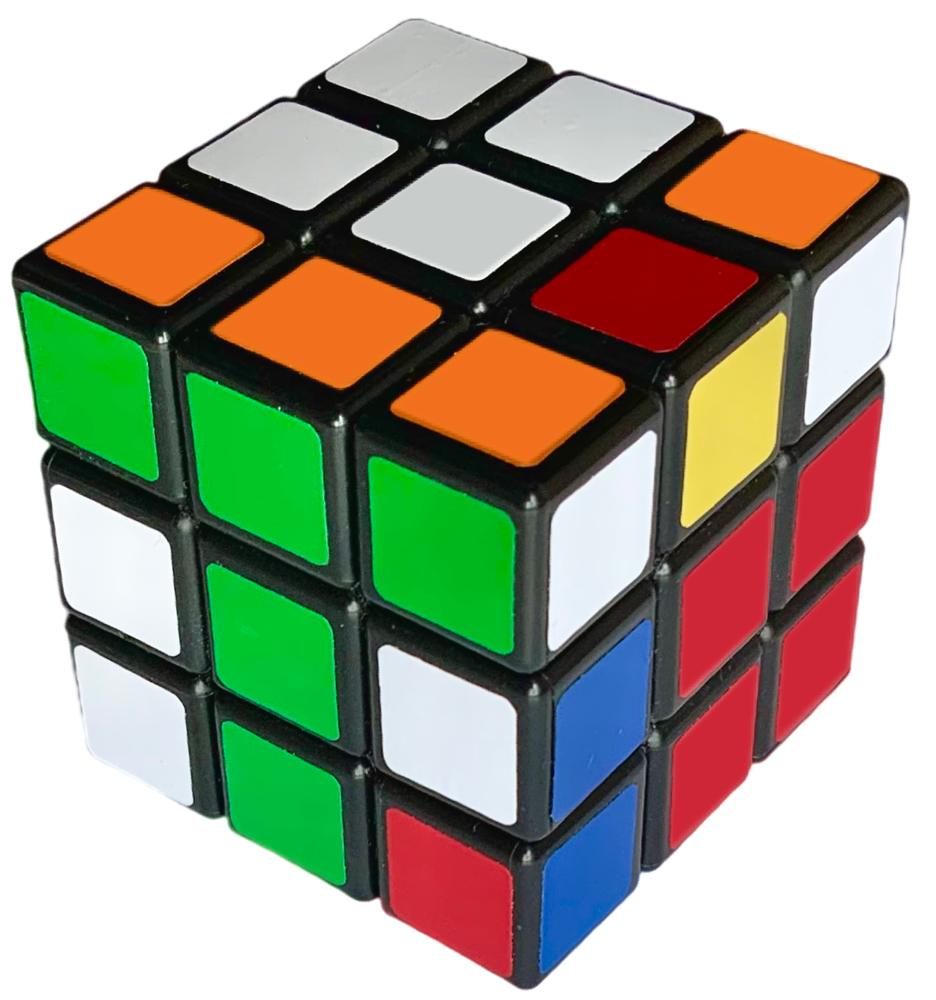
\includegraphics[height=0.75\textheight]{Bilder/Wuerfel_gerade_ausgeschnitten.png}
\end{frame}

\begin{frame}{Der Lösbarkeitssatz}
	\begin{satzbox*}{}{}
		Ein Würfel in Konfiguration 
		\[
			(\varphi, \rho, x, y) \in S_8 \times S_{12} \times (\ZZ/3\ZZ)^8 \times (\ZZ/2\ZZ)^{12}
		\]
		ist genau dann lösbar, wenn gilt: 
		\begin{enumerate} \setlength\parskip{5pt}
			\item[a)] \(\sgn(\varphi) = \sgn(\rho)\),
			\item[b)] \(\sum_{i=1}^8 x_i = x_1 + x_2 + \ldots + x_8\) ist durch 3 teilbar, 
			\item[c)] \(\sum_{j=A}^{L} y_j = y_A + y_B + \ldots + y_L\) ist durch 2 teilbar. 
		\end{enumerate}
	\end{satzbox*}
\end{frame}

\begin{frame}{Ist unser Würfel lösbar?}
	Die Konfiguration dieses Würfels:  \\[6pt]
	
	\begin{minipage}{0.53\textwidth}    
		\begin{itemize}
			\item \(\varphi =\) (1 2 5) (3 4) (6 7)
			\item \(\rho =\) (A E) (B C F J)
			\item \(x = (1,2,1,0,1,0,1,0)\)
			\item \(y = (1,1,1,0,0,0,0,0,0,1,0,0)\)
		\end{itemize}    
		
		\vspace{3mm}
		
		
		\begin{rememberbox}
			Die Bedingungen:
			\begin{itemize}
				\item[a)] \(\sgn(\varphi) = \sgn(\rho)\),
				\item[b)] \(\sum_{i=1}^8 x_i\) ist durch 3 teilbar, 
				\item[c)] \(\sum_{j=A}^{L} y_j\) ist durch 2 teilbar. 
			\end{itemize}
		\end{rememberbox}
	\end{minipage}
	\begin{minipage}{0.45\textwidth}
		\begin{figure}
			\flushright
			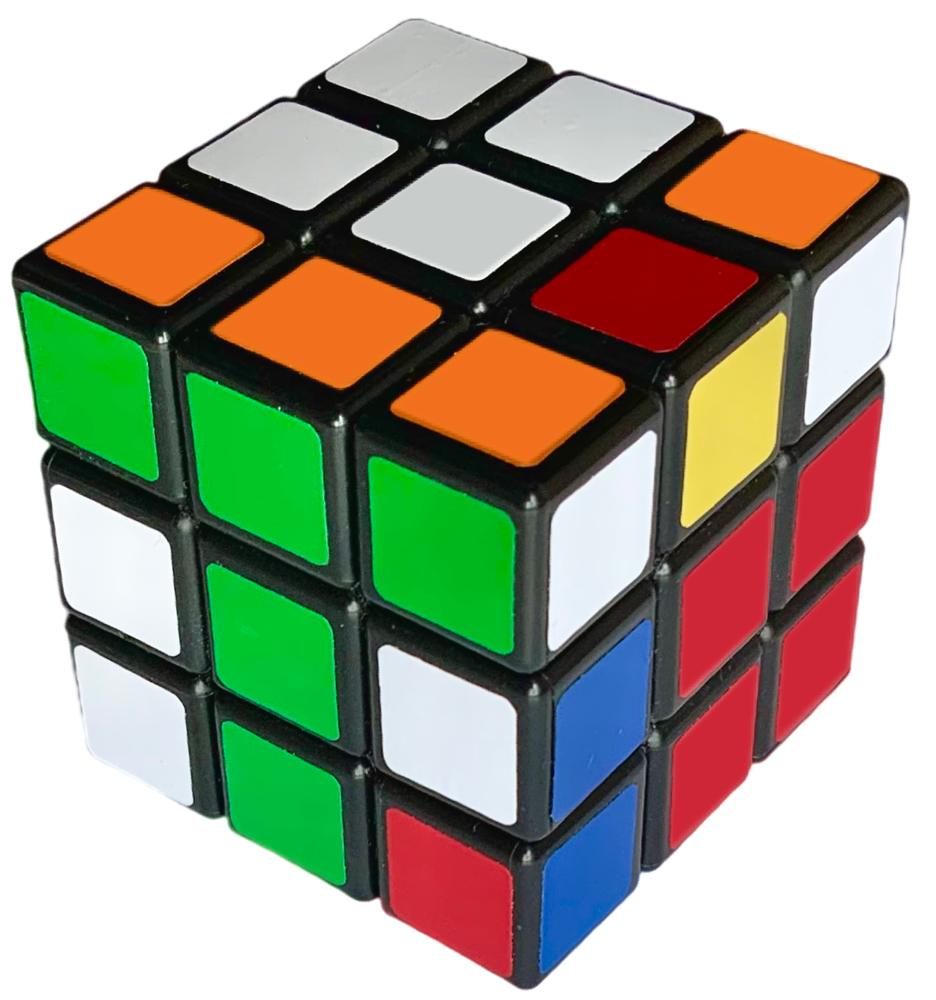
\includegraphics[width=4.5cm]{Bilder/Wuerfel_gerade_ausgeschnitten.png} 
		\end{figure}
	\end{minipage}
	
\end{frame}

\begin{frame}{Der Lösbarkeitssatz}
	\begin{satzbox*}{}{}
		Ein Würfel in Konfiguration 
		\[
		(\varphi, \rho, x, y) \in S_8 \times S_{12} \times (\ZZ/3\ZZ)^8 \times (\ZZ/2\ZZ)^{12}
		\]
		ist genau dann lösbar, wenn gilt: 
		\begin{enumerate} \setlength\parskip{5pt}
			\item[a)] \(\sgn(\varphi) = \sgn(\rho)\),
			\item[b)] \(\sum_{i=1}^8 x_i = x_1 + x_2 + \ldots + x_8\) ist durch 3 teilbar, 
			\item[c)] \(\sum_{j=A}^{L} y_j = y_A + y_B + \ldots + y_L\) ist durch 2 teilbar. 
		\end{enumerate}
	\end{satzbox*}
\end{frame}

\begin{frame}{Zum Beweis des Lösbarkeitssatzes}
	Wir müssen zwei Richtungen zeigen: 
	
	\vspace{15pt} 
	
	\begin{enumerate} \setlength\parskip{20pt}
		\item Wenn der Zauberwürfel lösbar ist, dann gelten a), b) und c). 
		\item Wenn a), b) und c) gelten, dann ist der Würfel lösbar (egal, wie er gerade aussieht).
	\end{enumerate}
\end{frame}

\begin{frame}{}
	\centering
	\beamerblue{\Large{Kurzvariante: Beweisidee}}
\end{frame}


\begin{frame}{Hinrichtung: Strategie}
	\begin{enumerate}\setlength\parskip{7pt}
		\item \green{Zeige:} Im Grundzustand \(c_0\) gilt die Eigenschaft.
		\item Wir nehmen an, wir sind in einem Zustand, in dem die Eigenschaft gilt.\\
			\green{Zeige:} Durch das Drehen einer Scheibe bleibt die Eigenschaft erhalten.
		\item Lösbarer Würfel ist durch Drehungen aus \(c_0\) entstanden\\
		\(\Rightarrow\) Eigenschaft gilt für lösbaren Würfel
	\end{enumerate}
	
	\begin{figure}
		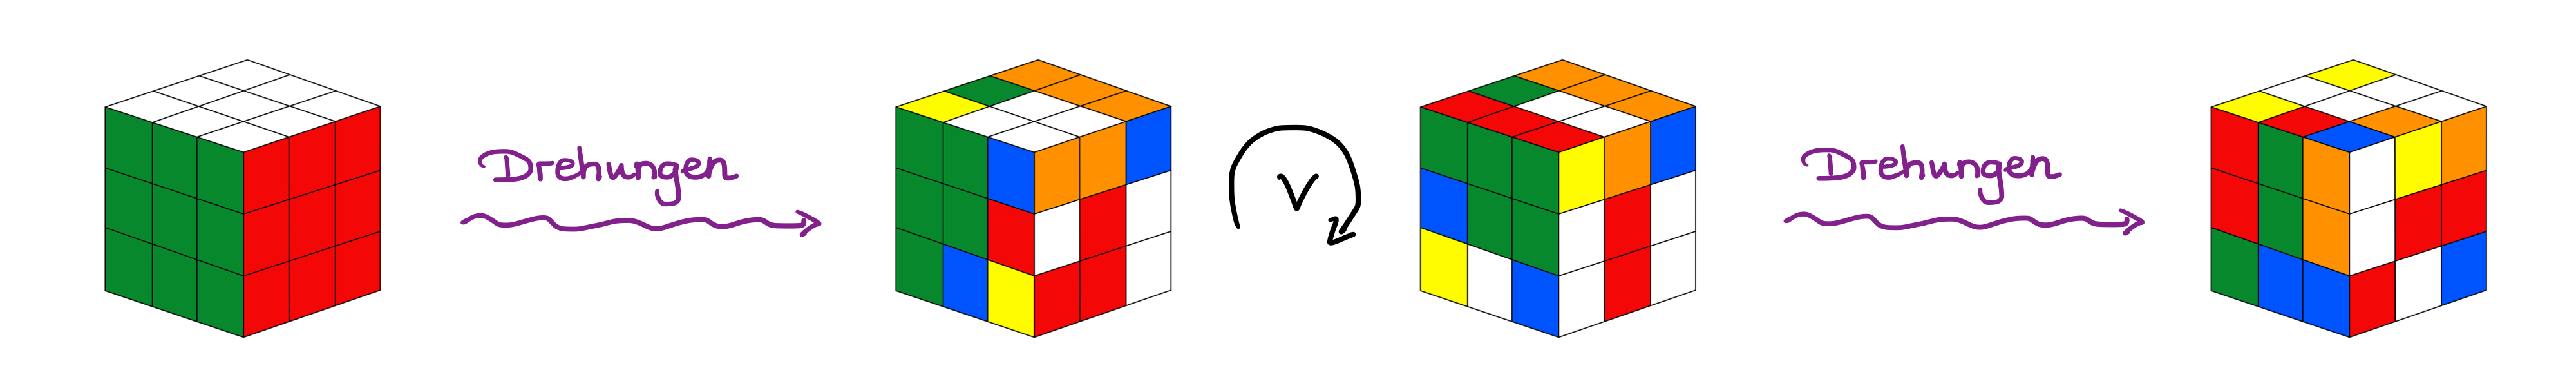
\includegraphics[width=\textwidth]{Bilder/Zauberwuerfel-Loesungsstrategie-Hinrichtung.png}
%		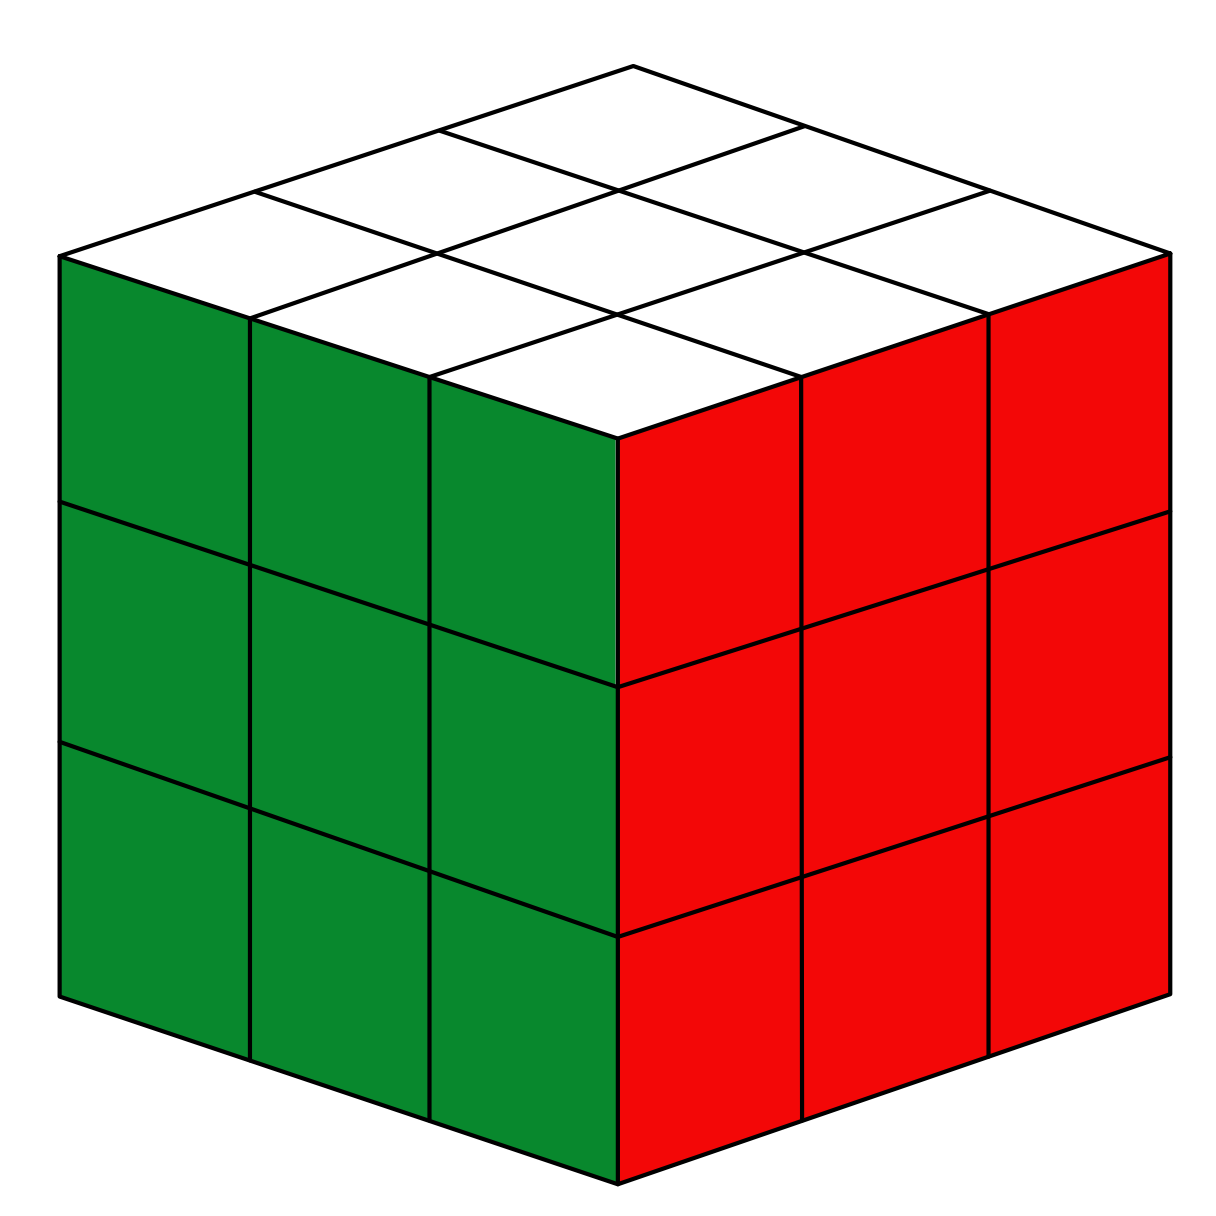
\includegraphics[height=1.7cm]{Bilder/Zauberwürfel-gemalt-grundzustand.png} 
%		\hspace{2.5cm}
%		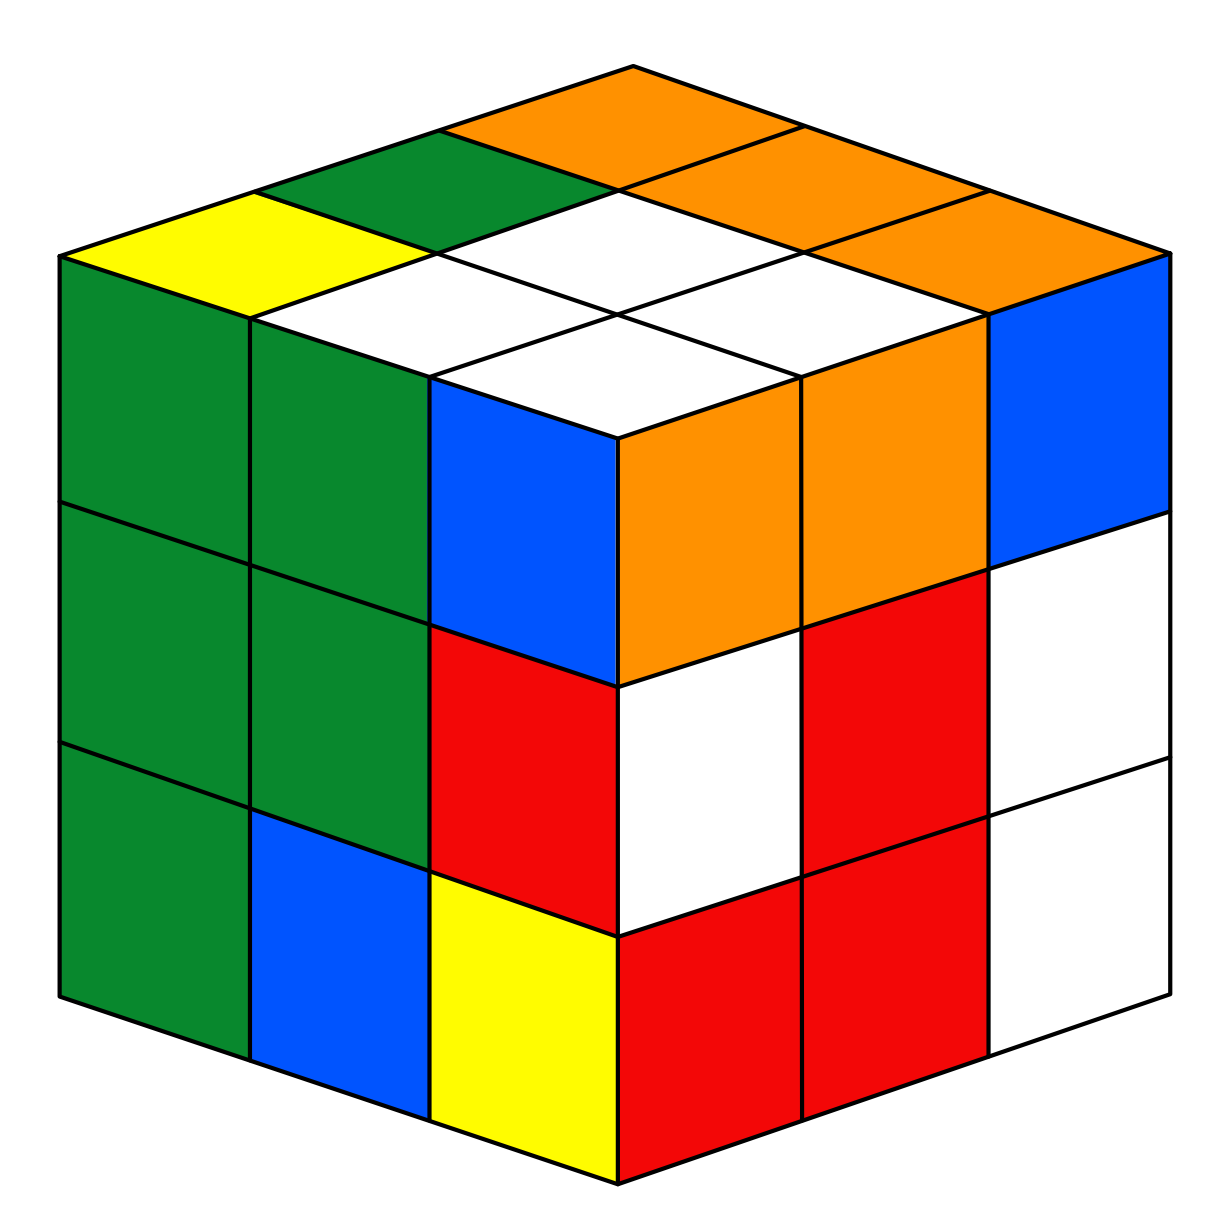
\includegraphics[height=1.7cm]{Bilder/Zauberwürfel-gemalt-bunt.png}  \(\overset{V}{\longrightarrow}\)\hspace{1cm}
%		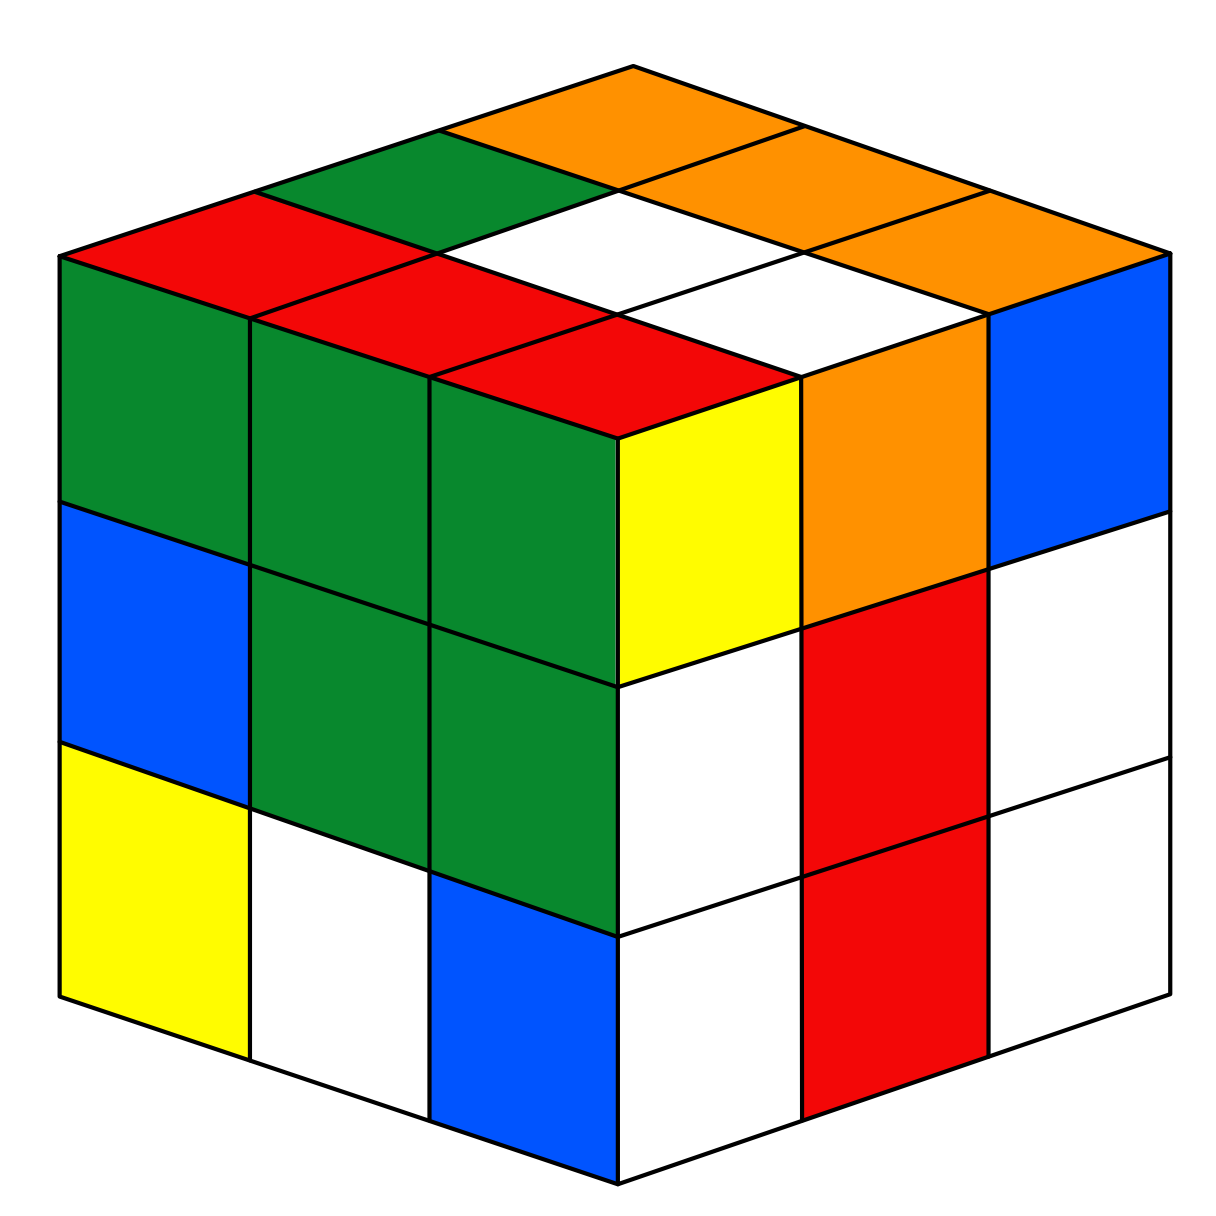
\includegraphics[height=1.7cm]{Bilder/Zauberwürfel-gemalt-bunt-gedreht.png} 
%		\hspace{2.5cm}
%		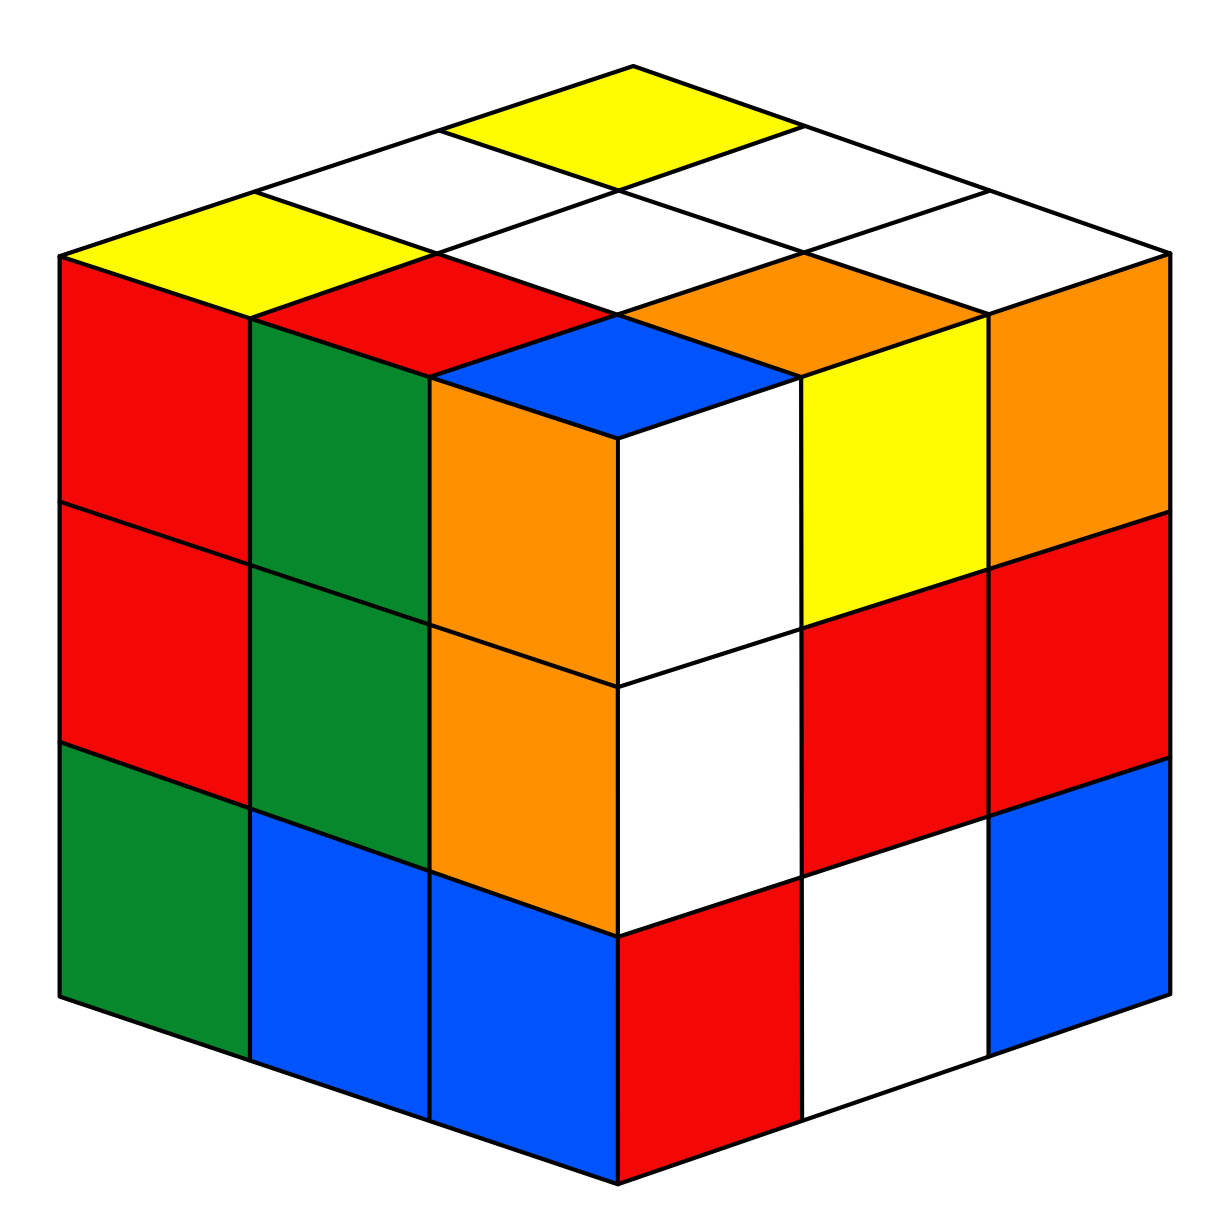
\includegraphics[height=1.7cm]{Bilder/Zauberwürfel-gemalt-bunt-loesbar.png} 
	\end{figure}
%	\small{Zeige:} \hspace{3.3cm} \small{Angenommen:} \hspace{1cm} \small{Zeige:} \hspace{2.7cm} \small{Lösbarer Würfel:}\\
%	\small{Eigenschaft gilt} \hspace{1.9cm} \small{Eigenschaft gilt} \hspace{0.8cm} \small{Eigenschaft gilt} \hspace{1.4cm} \small{Eigenschaft gilt}
\end{frame}

\begin{frame}{Strategie: a), b), c) gelten \(\Rightarrow\) Würfel ist lösbar}
	Wir nehmen an, dass die Bedingungen a), b) und c) gelten. 
	
	\vspace{7mm}
	
	Konstruiere allgemeines Manöver \(M\), das den Würfel zurück dreht (abhängig vom Aussehen vom Würfel)
	
	\vspace{7mm}
	
	Nutze: 
	\begin{itemize}
		\item[] a) \(\rightarrow\) Ecken und Kanten gleichzeitig an richtige Position bringen
		\item[] b) \(\rightarrow\) Ecken richtig drehen
		\item[] c) \(\rightarrow\) Kanten richtig drehen
	\end{itemize}
\end{frame}


\begin{frame}{}
	\centering
	\beamerblue{\Large{Langvariante: Beweis}}
\end{frame}

\begin{frame}{Hinrichtung: Strategie}
	\begin{enumerate}\setlength\parskip{7pt}
		\item \green{Zeige:} Im Grundzustand \(c_0\) gilt die Eigenschaft.
		\item Wir nehmen an, wir sind in einem Zustand, in dem die Eigenschaft gilt.\\
		\green{Zeige:} Durch das Drehen einer Scheibe bleibt die Eigenschaft erhalten.
		\item Lösbarer Würfel ist durch Drehungen aus \(c_0\) entstanden\\
		\(\Rightarrow\) Eigenschaft gilt für lösbaren Würfel
	\end{enumerate}
	
	\begin{figure}
		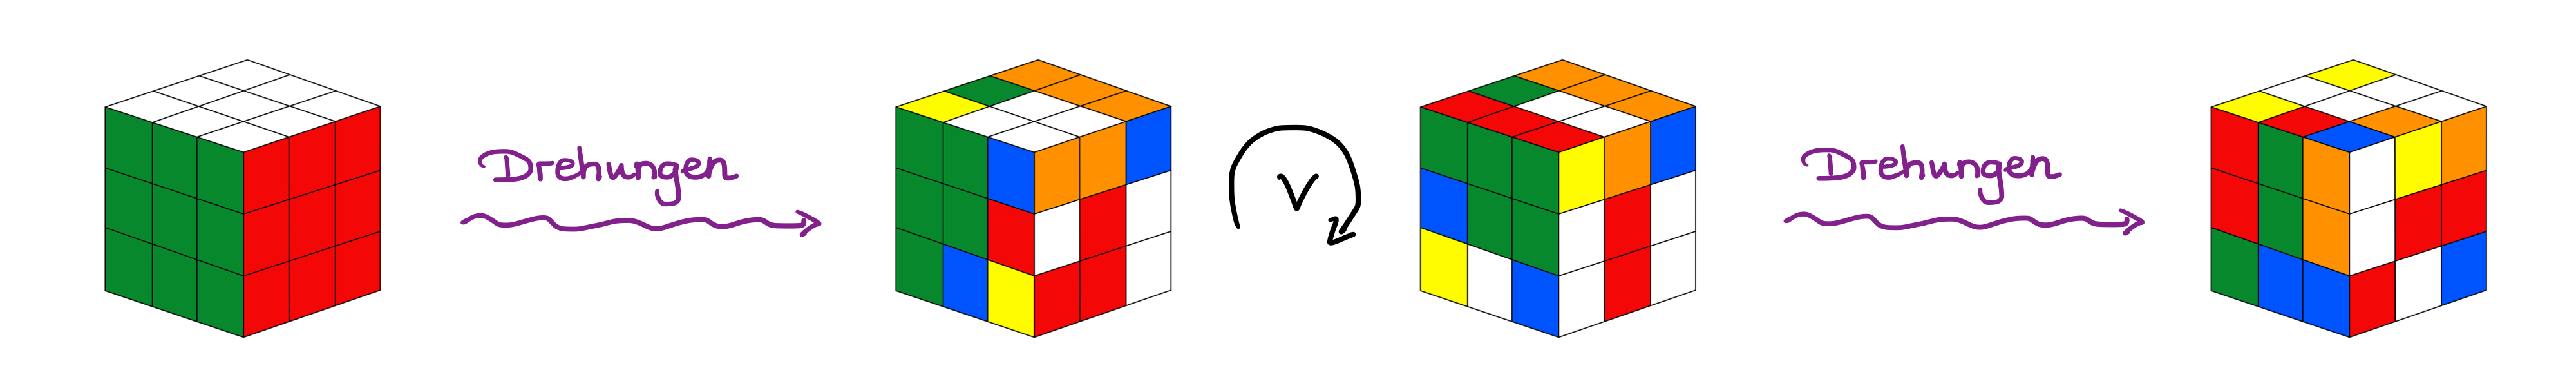
\includegraphics[width=\textwidth]{Bilder/Zauberwuerfel-Loesungsstrategie-Hinrichtung.png}
		%		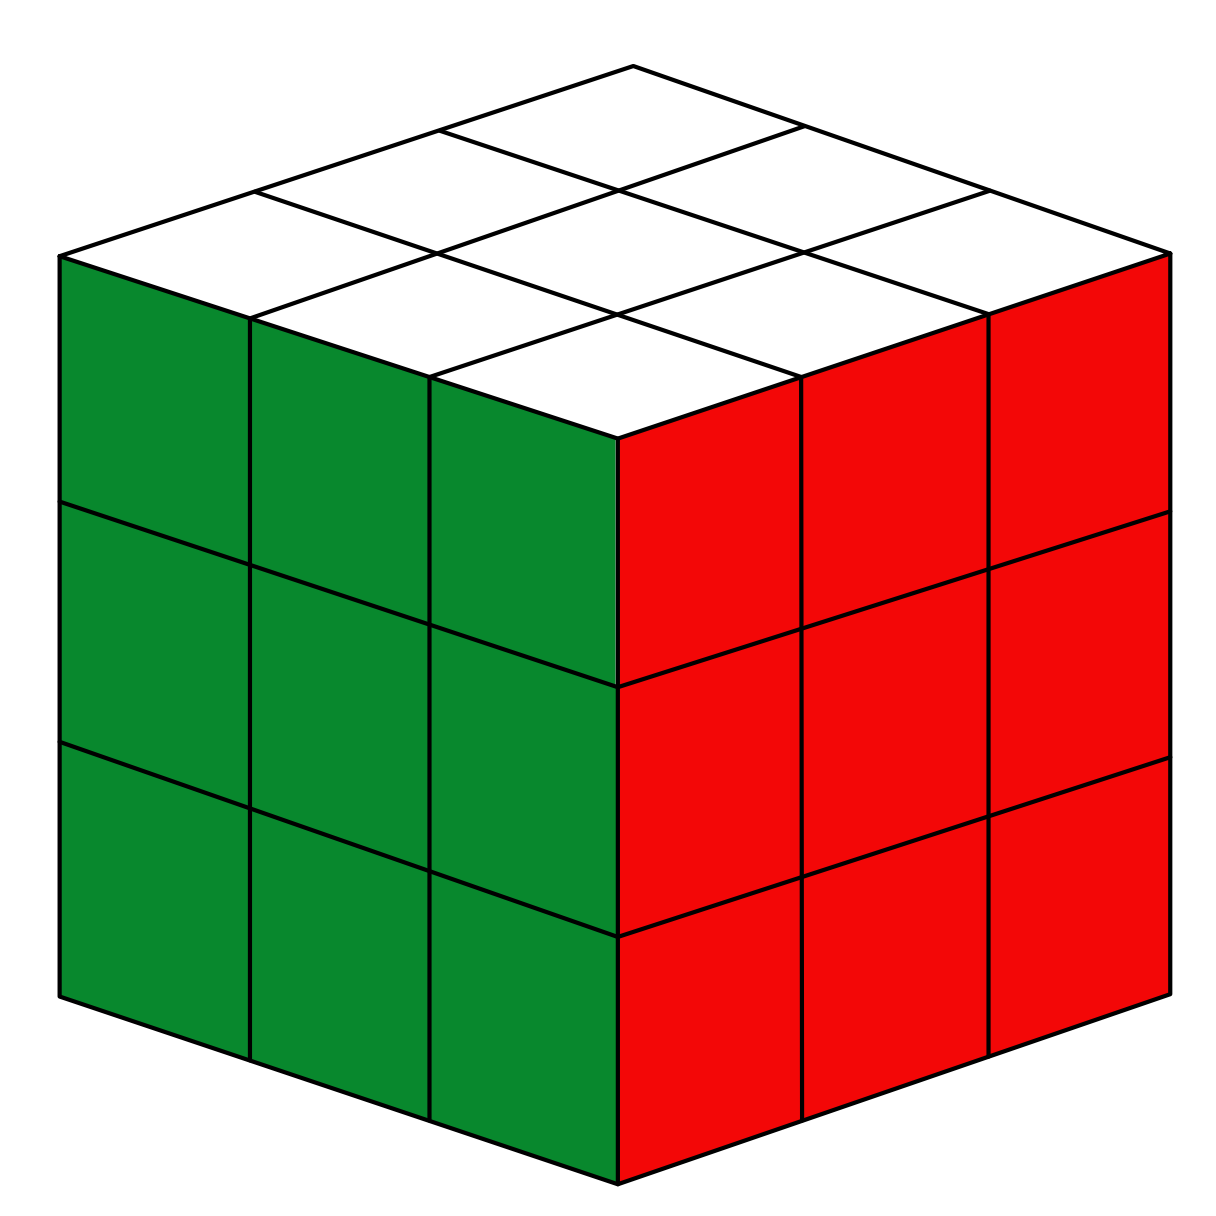
\includegraphics[height=1.7cm]{Bilder/Zauberwürfel-gemalt-grundzustand.png} 
		%		\hspace{2.5cm}
		%		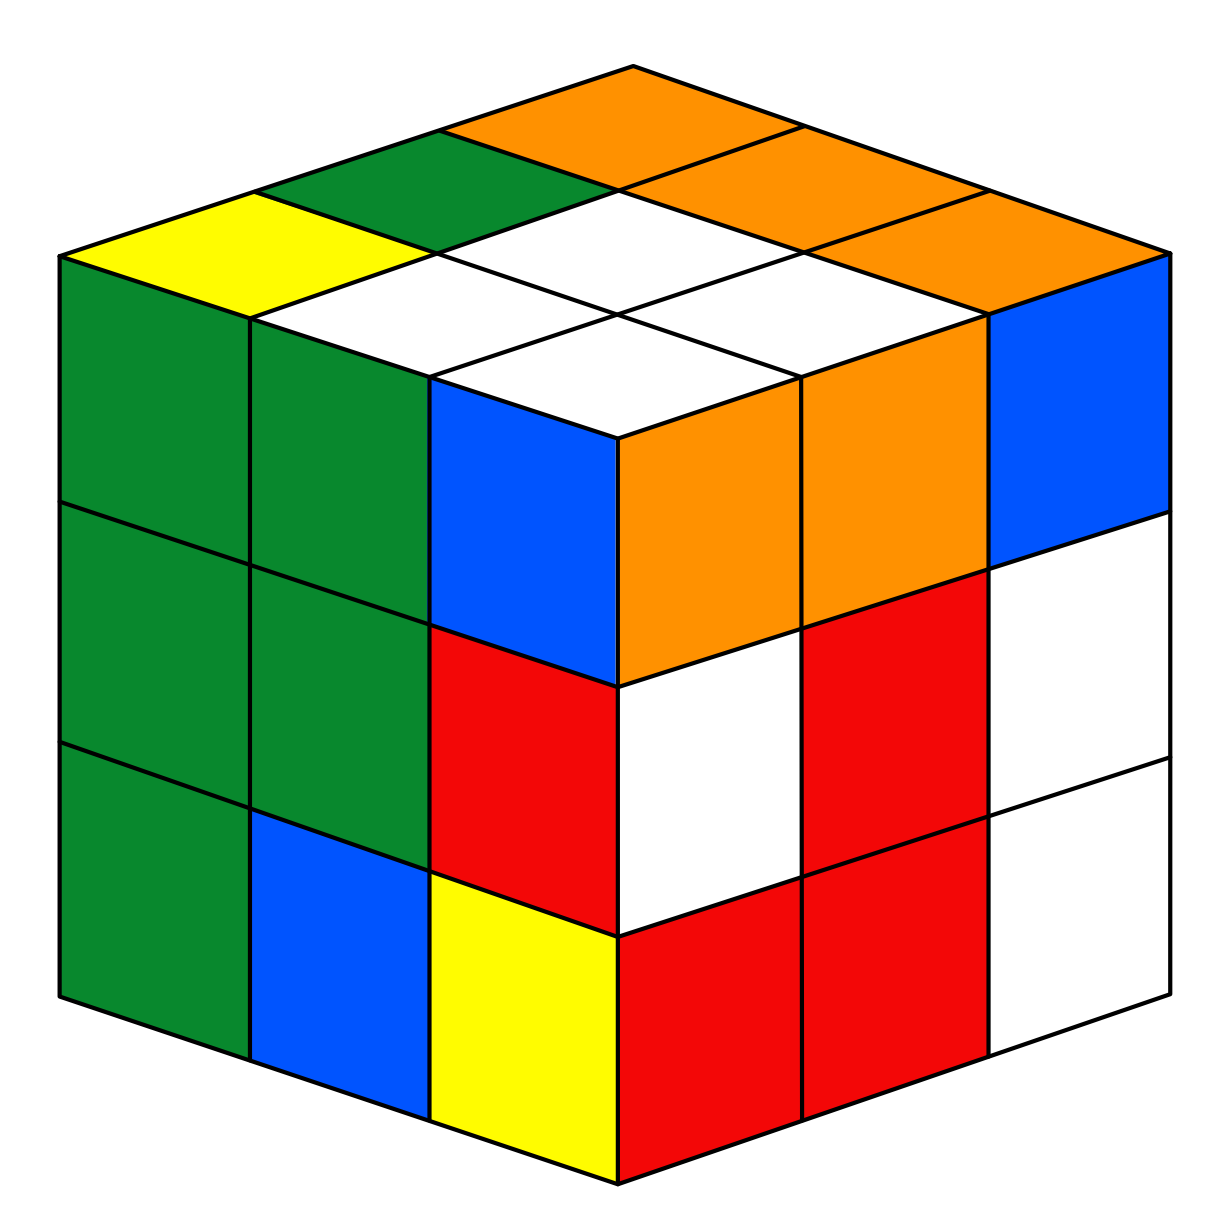
\includegraphics[height=1.7cm]{Bilder/Zauberwürfel-gemalt-bunt.png}  \(\overset{V}{\longrightarrow}\)\hspace{1cm}
		%		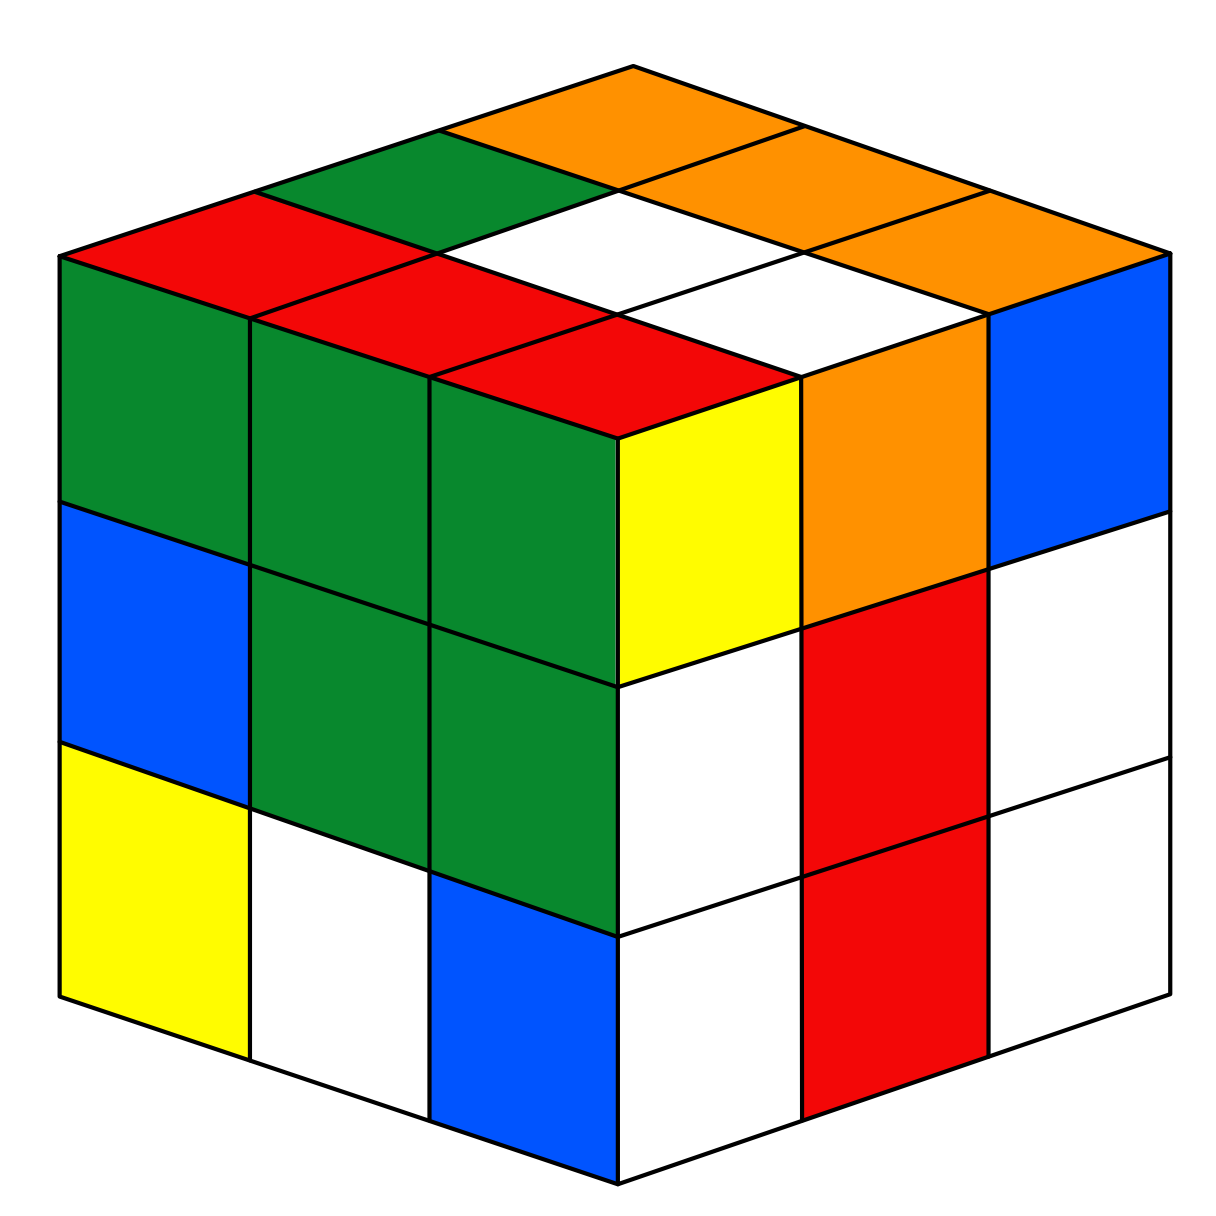
\includegraphics[height=1.7cm]{Bilder/Zauberwürfel-gemalt-bunt-gedreht.png} 
		%		\hspace{2.5cm}
		%		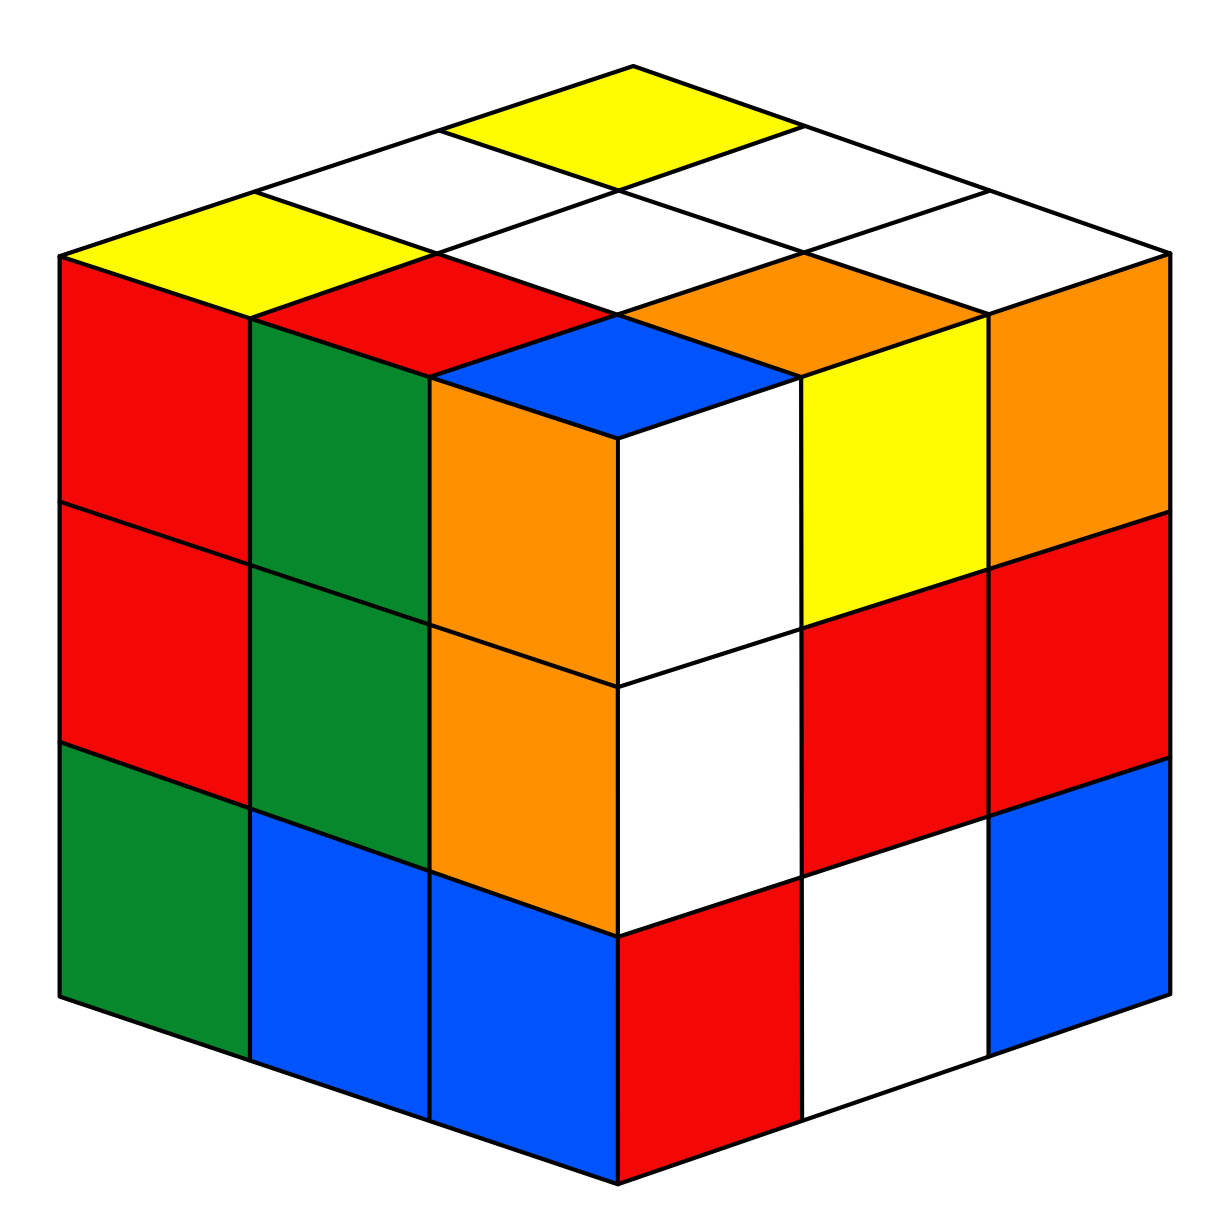
\includegraphics[height=1.7cm]{Bilder/Zauberwürfel-gemalt-bunt-loesbar.png} 
	\end{figure}
\end{frame}

\begin{frame}{Hinrichtung: b) \(\sum_{i=1}^8 x_i\) ist durch 3 teilbar}
     Im \textbf{Grundzustand} \(c_0\) haben alle Ecken die Orientierung 0, d.h. \(x = (0,\ldots, 0)\). 
     \[
         \sum_{i = 1}^8 x_i = 0. 
     \]

     \vspace{0.8cm}

     \textbf{Drehung:}

     Sei nun der Würfel beliebig verdreht und gelte \(\sum_i x_i\) ist durch 3 teilbar. Wir müssen zeigen, dass sich durch eine Drehung nichts an der Teilbarkeit der Summe \(\sum_i x_i\) durch 3 ändert. 
\end{frame}

\begin{frame}{Hinrichtung: b) \(\sum_{i=1}^8 x_i\) ist durch 3 teilbar }
     %Bei der Drehung einer Randscheibe ändern sich die Orientierung aller Ecken nach einem bestimmten Schema: 
     Vor der Drehung: \(a + b + c + d + X\) ist durch 3 teilbar.

     %\vspace{6mm}

     \begin{figure}
	         \centering
	         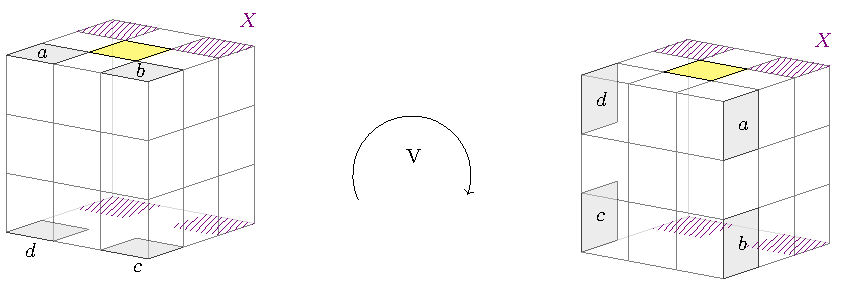
\includegraphics[scale=0.7]{Bilder/Wuerfel_Eckorientierung.pdf}
	     \end{figure}
	\pause
    Nach der Drehung gilt: \small{\(a + \left\{\begin{array}{c} 2 \\ -1 \end{array}\right\} + b + \left\{\begin{array}{c} 1 \\ -2 \end{array}\right\} + c + \left\{\begin{array}{c} 2 \\ -1 \end{array}\right\} + d + \left\{\begin{array}{c} 1 \\ -2 \end{array}\right\} + X\) \\[6pt] \pause
    \hspace{3.8cm} \(= a + b + c + d + \left\{\begin{array}{c} 3 \\ 0 \\ -3 \end{array}\right\} + \left\{\begin{array}{c} 3 \\ 0 \\ -3 \end{array}\right\}\) ist durch 3 teilbar}
     %\vspace{10mm}
\end{frame}



\begin{frame}{Strategie: a), b), c) gelten \(\Rightarrow\) Würfel ist lösbar}
Wir nehmen an, dass die Bedingungen a), b) und c) gelten. 

\vspace{7mm}

Konstruiere allgemeines Manöver \(M\), das den Würfel zurück dreht (abhängig vom Aussehen vom Würfel)

\vspace{7mm}

Nutze: 
\begin{itemize}
	\item[] a) \(\rightarrow\) Ecken und Kanten gleichzeitig an richtige Position bringen
	\item[] b) \(\rightarrow\) Ecken richtig drehen
	\item[] c) \(\rightarrow\) Kanten richtig drehen
\end{itemize}
\end{frame}

 \begin{frame}{Rückrichtung: Positionierung der Ecken}
      \begin{tcolorbox}[colback=ForestGreen!5!white,colframe=ForestGreen!75!black,title=Fakt]
	         Jede Drehung aus der \(A_n\) lässt sich als Produkt von Zykeln der Form \((1 \ 2 \ i)\) für \(i \in \{3, \ldots 8\}\) schreiben. 
	     \end{tcolorbox}
     \vspace{3mm}
     Da \(\sgn(\varphi) = 1\), ist \(\varphi \in A_{n}\). \\[4pt]
     Also gibt es \(i_1, i_2, \ldots, i_m \in \{3, \ldots, 8\}\), um \(\varphi\) zu schreiben als 
     \[
         \varphi = (1~2~i_1)~(1~2~i_2)~(1~2~i_3) \ldots (1~2~i_m).
     \]
     \textbf{Ziel:}\\
     Finde drehbares Manöver \(M_{iE} = (1~2~i)\) für jedes \(i \in \{3, \ldots, 8\}\). 
     % Jeder Zykel der Form \((1~2~i)\) mit \(i \in \{3, \ldots 8\}\) ist drehbar. 
     % Also lässt sich ein Manöver finden, um \(\varphi\) zurückzudrehen. \\[6pt]
     % \textbf{Alle Ecken sind nun an der richtigen Position.}
 \end{frame}


 \begin{frame}{Rückrichtung: Zutat 1 -  Das Manöver \(m_{VE}\)}
     Wir kennen bereits das Manöver
         \[
             m_{VE}: \quad  R~H^{-1}~R~V^2~R^{-1}~H~R~V^2~R^2
             %m_{VE}: \quad \rightarrow V O^{-1} H^{-1} O V^{-1} O^{-1} H O.
         \]  

     Wirkung: 
     \begin{itemize}
	         \item \(m_{VE}\) vertauscht genau die drei Ecken \(E_{1}, E_{2}\) und \(E_3\),
	         \item \(m_{VE}\) lässt die Kanten fest.
	     \end{itemize}
     \vspace{3mm}

     Mathematisch notiert: 
     \begin{align*}
	         m_{VE}^\me &= (1 \ 2 \ 3) \\
	         m_{VE}^\mk &= \id. 
	     \end{align*}

 \end{frame}

 \begin{frame}{Rückrichtung: Zutat 2 - Das Manöver \(m_i\)}
     \begin{minipage}{0.65\textwidth}
	     Für jede Ecke \(E_{i}\) mit \(i \in \{4,...,8\}\) gibt es ein Manöver
	
	        \begin{center}
		         \(m_{i}, \)
		         \end{center}
	
	     für das gilt:
	         \begin{itemize} \setlength\parskip{2pt}
		             \item \(m_i\) schickt Ecke \(E_i\) auf Position 3,
		             \item \(m_i\) lässt die Ecken auf Position 1 und 2 fest, 
		             % \item \(m_i\) vertauscht die Kanten irgendwie. 
		         \end{itemize}
	
	
	         % \vspace{3pt}
	         % Für die Ecken kann man \(m_i^\me\) schreiben als
	         % \[
	         %     m_{i}^\me=\widetilde{m}_{i}^\me \ (i \ 3),
	         % \]
	         % wobei \(\widetilde{m}_{i}^\me\) die Positionen 1,2,und 3 fest lässt. 
	         \end{minipage}
         \begin{minipage}{0.33\textwidth}
	             %\centering
	             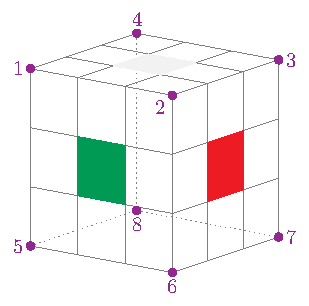
\includegraphics[width=0.89\textwidth]{Bilder/Wuerfel_Bezeichnungen_Ecken.pdf}
	         \end{minipage}

         \vspace{5mm}

          Die Kanten werden durch \(m_i\) irgendwie vertauscht. 
 \end{frame}
 
 \begin{frame}{Rückrichtung: Ecken - Das Manöver \(M_{iE}\)}
     Baue das Manöver \(M_{iE}=m_i^{-1}\ m_{VE} \ m_i\). \hspace{1.8cm} \small{\(i, w, x, y, z \in \{4, \ldots, 8\}\)} \\[13pt]
     \begin{minipage}{0.62\textwidth}    
	      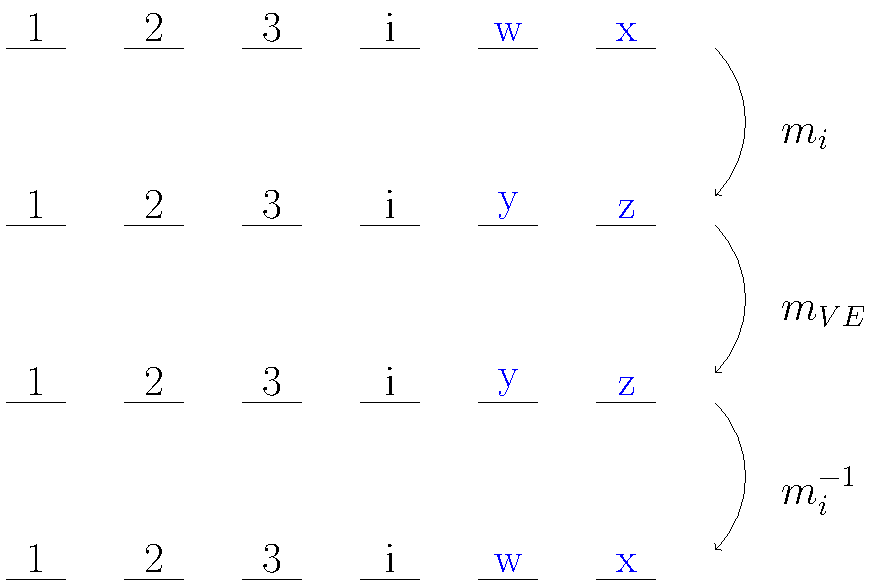
\includegraphics[width=0.95\textwidth]{Bilder/Hintereinanderausfuehrung_Beweis_M_iE.pdf}
	     \end{minipage}
     \begin{minipage}{0.36\textwidth}
	         \begin{small}
		             \begin{rememberbox}
			                 Erinnerung:%\\[5pt]
			                 \begin{itemize} \setlength\parskip{2pt}
			                     \item \(m_i^\me:\)  1 und 2 bleiben fest 
			                     \item \(m_i^\me:\) \(i\) \(\leadsto\) 3 
			                     \item \(m_i^\mk\) unbekannt 
			                 \end{itemize}
			                 \vspace{3mm}
			
			                 \begin{itemize}\setlength\parskip{2pt}
				                     \item \(m_{VE}^\me = (1~2~3)\) 
				                     \item \(m_{VE}^\mk = id\)
				                 \end{itemize}
			             \end{rememberbox}
		         \end{small}
	     \end{minipage}   
	     \vspace{4mm}
	     
	     \centering
	     \phantom{Das Manöver \(M_{iE}\) ist für jedes \(i \in \{3, \ldots, 8\}\) drehbar!}
 \end{frame}

 \begin{frame}{Rückrichtung: Ecken - Wirkung von \(M_{iE}\)}
     Das Manöver \(M_{iE}=m_i^{-1}\ m_{VE} \ m_i\). \hspace{1.8cm} \small{\(i, w, x, y, z \in \{4, \ldots, 8\}\)} \normalsize\\[5pt]
     \begin{minipage}{0.62\textwidth}    
	         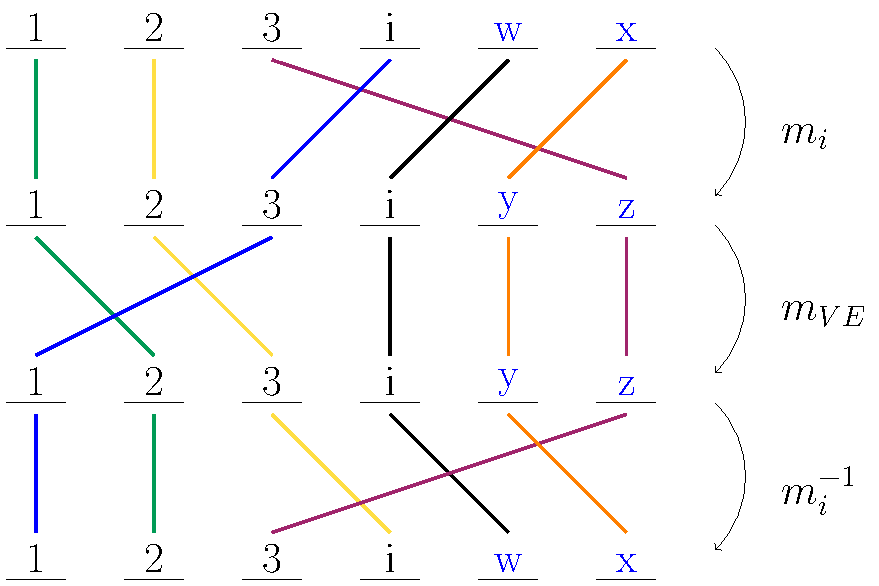
\includegraphics[width=0.9\textwidth]{Bilder/Zykel.pdf}
	     \end{minipage}
     \begin{minipage}{0.36\textwidth}
	         Wirkung:\\[5pt]
	         \begin{tabularx}{5cm}{ll}
		             \(M_{iE}^\me\) &= \((1~2~i)\)\\
		             & \\
		             \(M_{iE}^\mk\) &= \(\id\)
		         \end{tabularx}
	
	         \vspace{5mm}
	
	         % Wichtig: \\[5pt]
	         % Für jedes \(i \in \{3, \ldots, 8\}\) ist \\\(M_{iE}\) drehbar! 
	     \end{minipage}  
     \vspace{4mm}

     \centering
     Das Manöver \(M_{iE}\) ist für jedes \(i \in \{3, \ldots, 8\}\) drehbar! 
 \end{frame}


\begin{frame}{Rückrichtung: Orientierung der Ecken}
	\begin{minipage}{0.6\textwidth}
		\(m_{FE}\) dreht die Ecken 1 und 2 in verschiedene Richtungen:
		\[
		% m_{FE}=R^{-1}(R^{-1}VU^{2}V^{-1}RO^{2})^{2}R % wenn man von rechts nach links liest
		m_{FE} :\quad  \rightarrow R \left ( O^2 R V^{-1} U^2 V R^{-1} \right)^2 R^{-1} % wenn man von links nach rechts dreht
		\]
		Bedingung b): 
		\[x_1 + x_2 + \ldots + x_7 + x_8 \text{ ist durch 3 teilbar.} \]  
		
		\vspace{0.5cm}
		
		
	\end{minipage}
	\begin{minipage}{0.38\textwidth}
		\flushright
		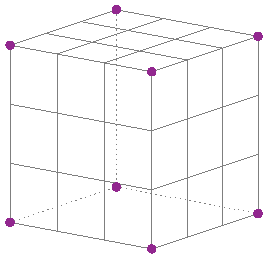
\includegraphics[width=0.85\textwidth]{Bilder/Wuerfel_simpel.pdf}
	\end{minipage}
	\(\leadsto\) Sind 7 Ecken richtig orientiert,  dann automatisch auch die 8. 
\end{frame}

\begin{frame}{Rückrichtung: Orientierung der Kanten}
	\begin{minipage}{0.6\textwidth}
		\(m_{FK}\) flippt die Kanten A und B:             
		\[
		%m_{FK}=RO^{2}R^{2}O^{-1}RORO^{2}L^{-1}V^{-1}R^{-1}VL  %wenn man von rechts nach links liest\\
		m_{FK}: \quad  \rightarrow   L V R^{-1} V^{-1} L^{-1} O^2 R O R O^{-1} R^2 O^2 R %wenn man von links nach rechts liest
		\]
		Bedingung c):
		\[y_1 + y_2 + \ldots + y_{11} + y_{12} \text{ ist durch 2 teilbar.} \] 
	\end{minipage}
	\begin{minipage}{0.38\textwidth}
		\flushright
		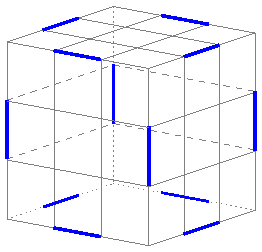
\includegraphics[width=0.82\textwidth]{Bilder/Wuerfel_simpel_Kanten.pdf}
	\end{minipage}    
	
	\(\leadsto\) Sind 11 Kanten richtig orientiert, dann automatisch auch die 12. 
	
	
	\vspace{5mm}
	\textbf{Und damit ist der Würfel gelöst!}
\end{frame}

\begin{frame}
	\centering
	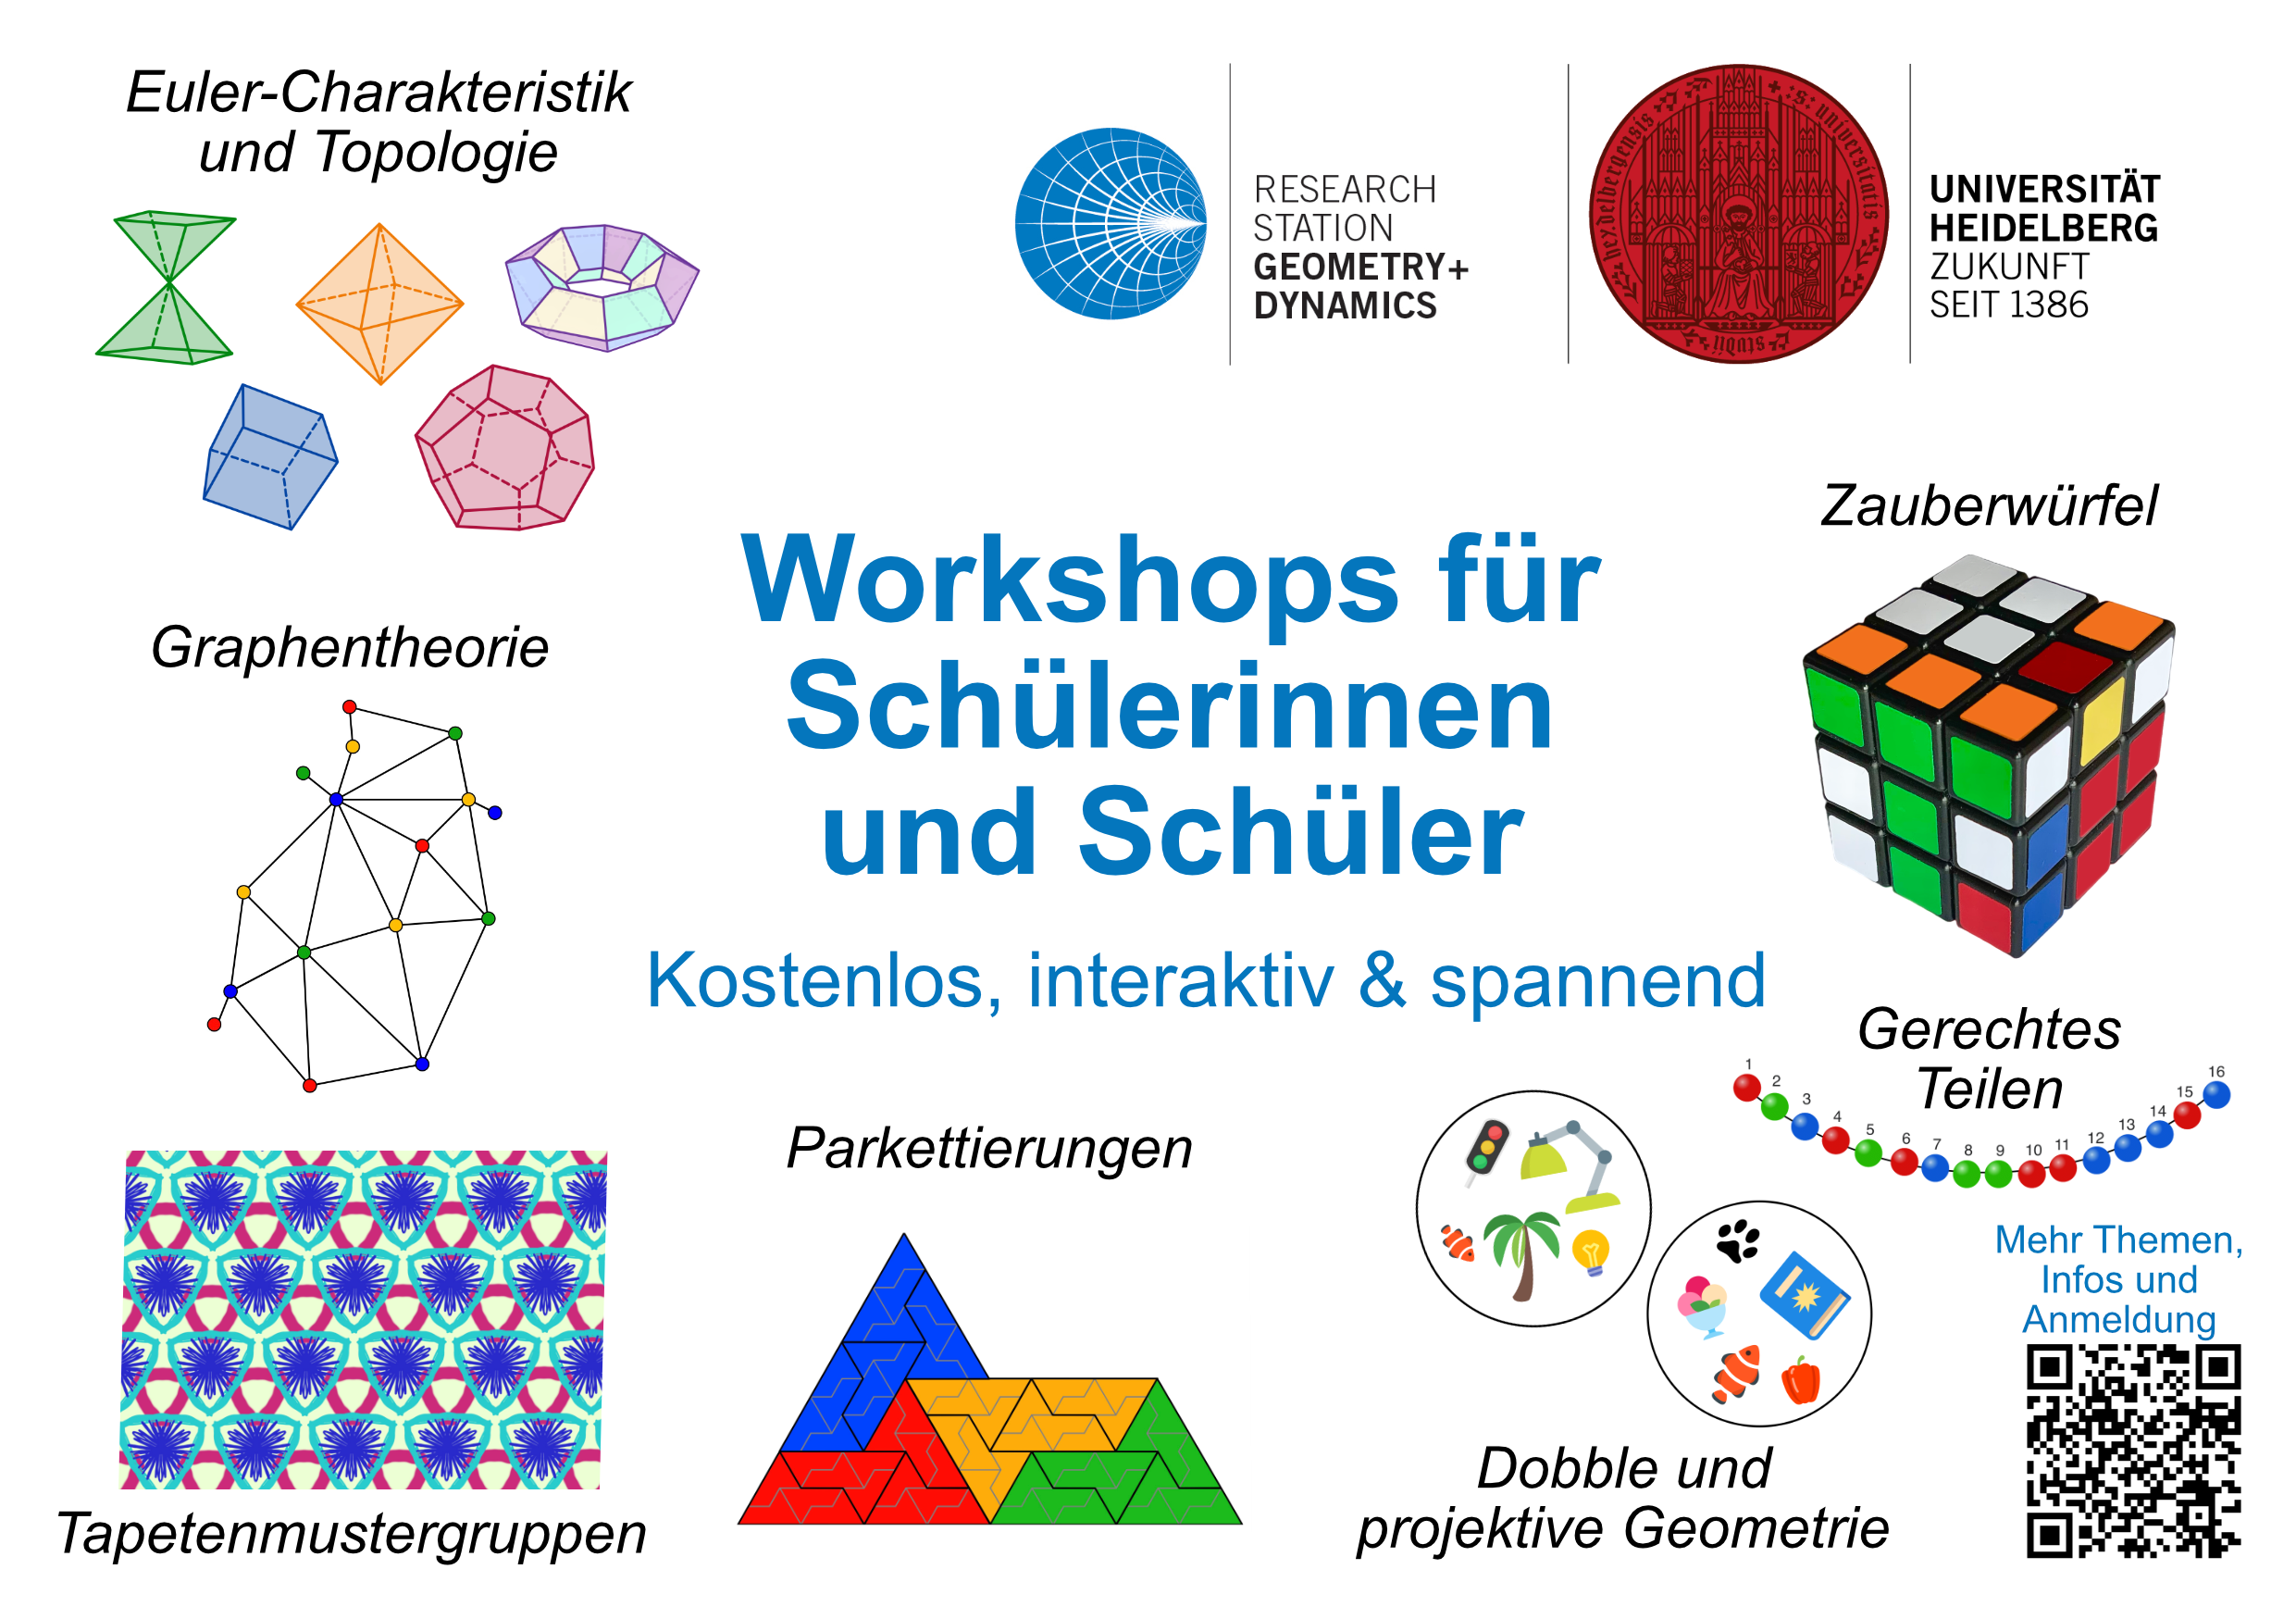
\includegraphics[height=\textheight]{Bilder/Flyer.png}
\end{frame}



\end{document}